%%%%%%%%%%%%%%%%%%%%%%%%%%%%%%%%%%%%%%%%%%%%%%%%%%%%%%%%%%%%%%%%%%%%%%
% Edit the title below to update the display in My Documents
%\title{Project Report}
%
%%% Preamble
\documentclass[paper=a4, fontsize=11pt]{scrartcl}
\usepackage[T1]{fontenc}
\usepackage{fourier}

\usepackage[english]{babel}															% English language/hyphenation
\usepackage[protrusion=true,expansion=true]{microtype}	
\usepackage{amsmath,amsfonts,amsthm} % Math packages
\usepackage[pdftex]{graphicx}	
\usepackage{url}
\usepackage{color}
\usepackage{graphicx}
\usepackage[dvipsnames]{xcolor}
\usepackage{subfig}
\usepackage{float}

\usepackage{alphalph}
\renewcommand*{\thesubfigure}{%
\alphalph{\value{subfigure}}%
}

%%% Custom sectioning
\usepackage{sectsty}
\allsectionsfont{\centering \normalfont\scshape}


%%% Custom headers/footers (fancyhdr package)
\usepackage{fancyhdr}
\pagestyle{fancyplain}
\fancyhead{}											% No page header
\fancyfoot[L]{}											% Empty 
\fancyfoot[C]{}											% Empty
\fancyfoot[R]{\thepage}									% Pagenumbering
\renewcommand{\headrulewidth}{0pt}			% Remove header underlines
\renewcommand{\footrulewidth}{0pt}				% Remove footer underlines
\setlength{\headheight}{13.6pt}

%%% Insert hyperlinks
\usepackage{hyperref} 

%%% Equation and float numbering
\numberwithin{equation}{section}		% Equationnumbering: section.eq#
\numberwithin{figure}{section}			% Figurenumbering: section.fig#
\numberwithin{table}{section}				% Tablenumbering: section.tab#


%%% Maketitle metadata
\newcommand{\horrule}[1]{\rule{\linewidth}{#1}} 	% Horizontal rule

\title{
		%\vspace{-1in} 	
		\usefont{OT1}{bch}{b}{n}
		\normalfont \normalsize \textsc{IITM-CS4011 : Principles of Machine Learning} \\ [25pt]
		\horrule{0.5pt} \\[0.4cm]
		\huge Programming Assignment 3 \\
		\horrule{2pt} \\[0.5cm]
}
\author{
		\normalfont 								\normalsize
        EE15B025 : Ganga Meghanath\\[-3pt]		\normalsize
        \today
}
\date{}


%%% Begin document
\begin{document}
\maketitle
\section*{CLUSTERING}
Clustering is the task of dividing the population or data points into a number of groups such that data points in the same groups are more similar to other data points in the same group than those in other groups.Eight 2-dimensional datasets have been provided for clustering: Aggregation, Compound, Path-based, Spiral, D31, R15, Jain, Flames. First two columns are the features and the third column is the class label. Various analysis and visualisations have been conducted on the same and the observations and results recorded.
\subsection*{1.Conversion of data into ARFF format}
The conversion has been done using Weka. The python code for the manual conversion is present in \textcolor{Brown}{Code->q1->arff.py}. The folder structure is depicted as follows :

\begin{center}
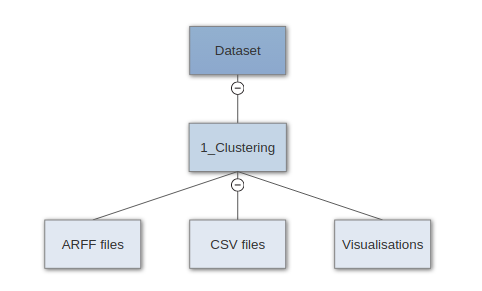
\includegraphics[scale=0.55]{Dataset_graph}
\end{center}

\subsection*{2.Visualisation}
All the visualisations have been done using Weka. The histograms have been color-coded according to the class-labels (last column). The first two columns are features f1 and f2 respectively.
\graphicspath{ {../Dataset/1_Clustering/Visualisations/} }

\subsubsection*{(i)Aggregation}
\begin{figure}[H]
  \centering
  \subfloat{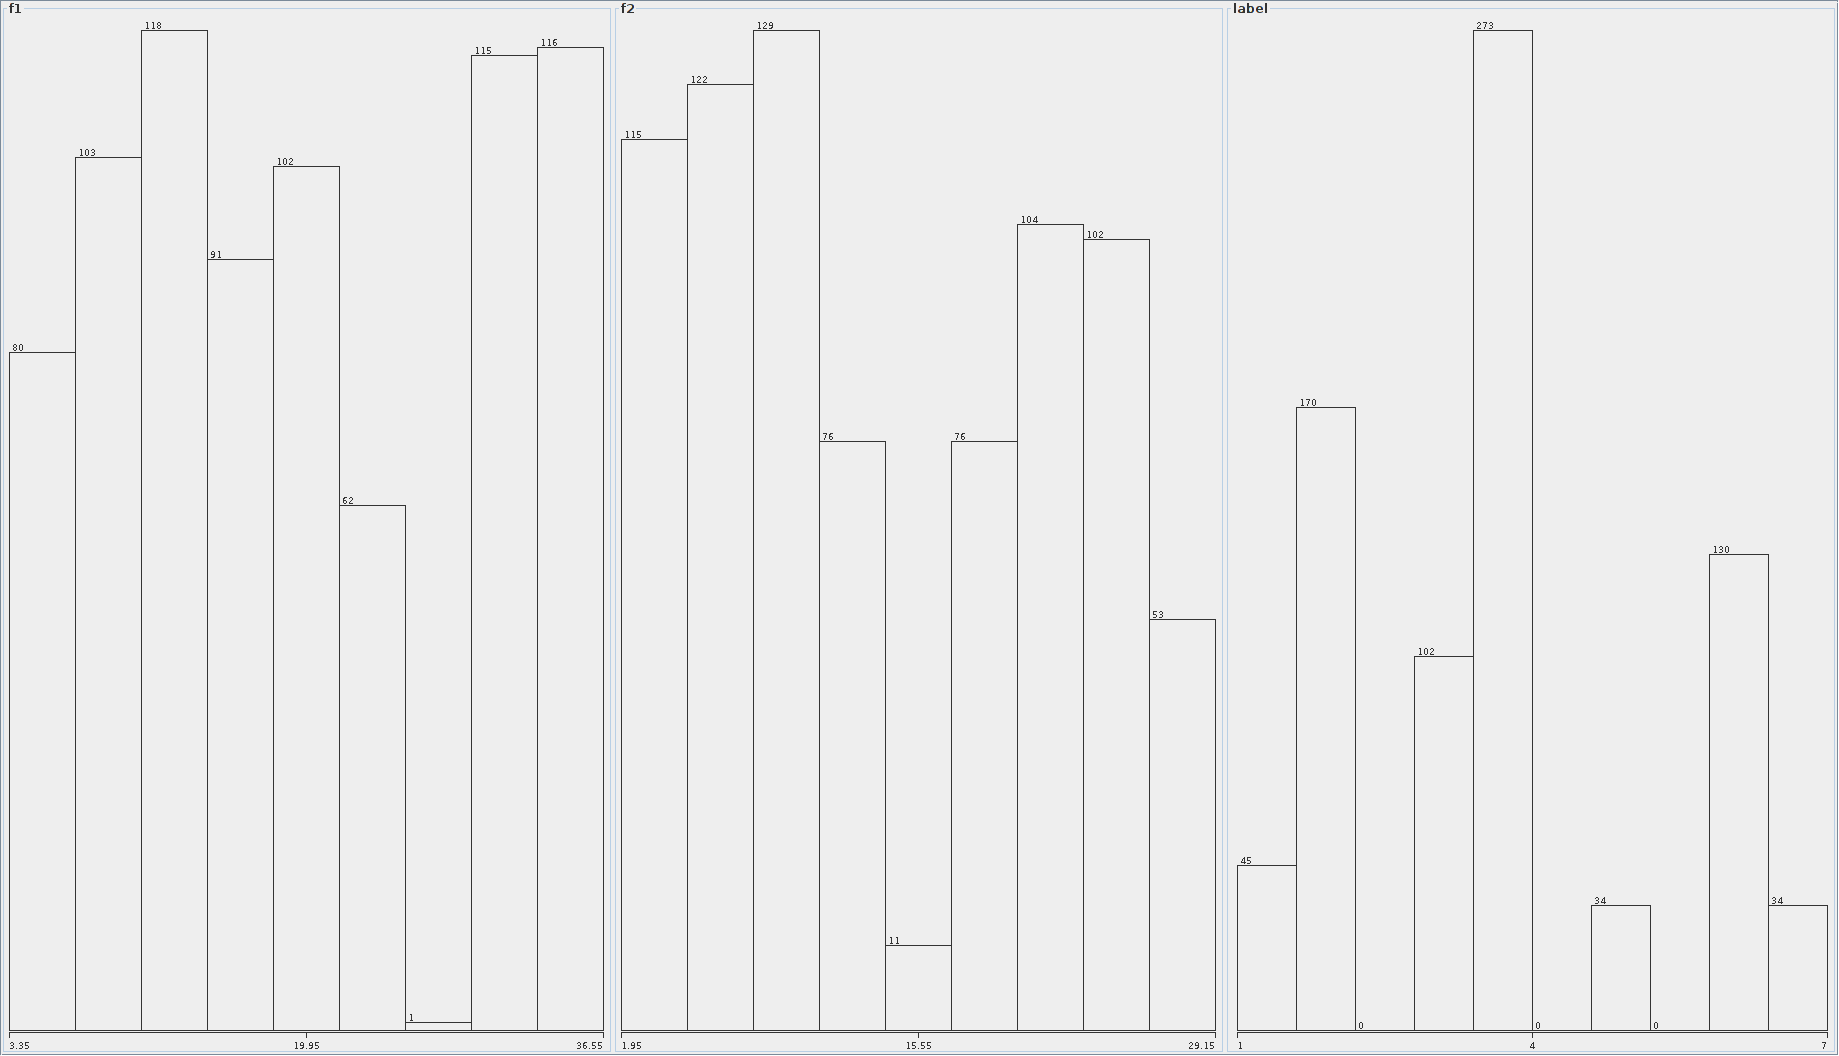
\includegraphics[width=0.7\textwidth]{Aggregation}\label{fig:f1}}
  \hfill
  \subfloat{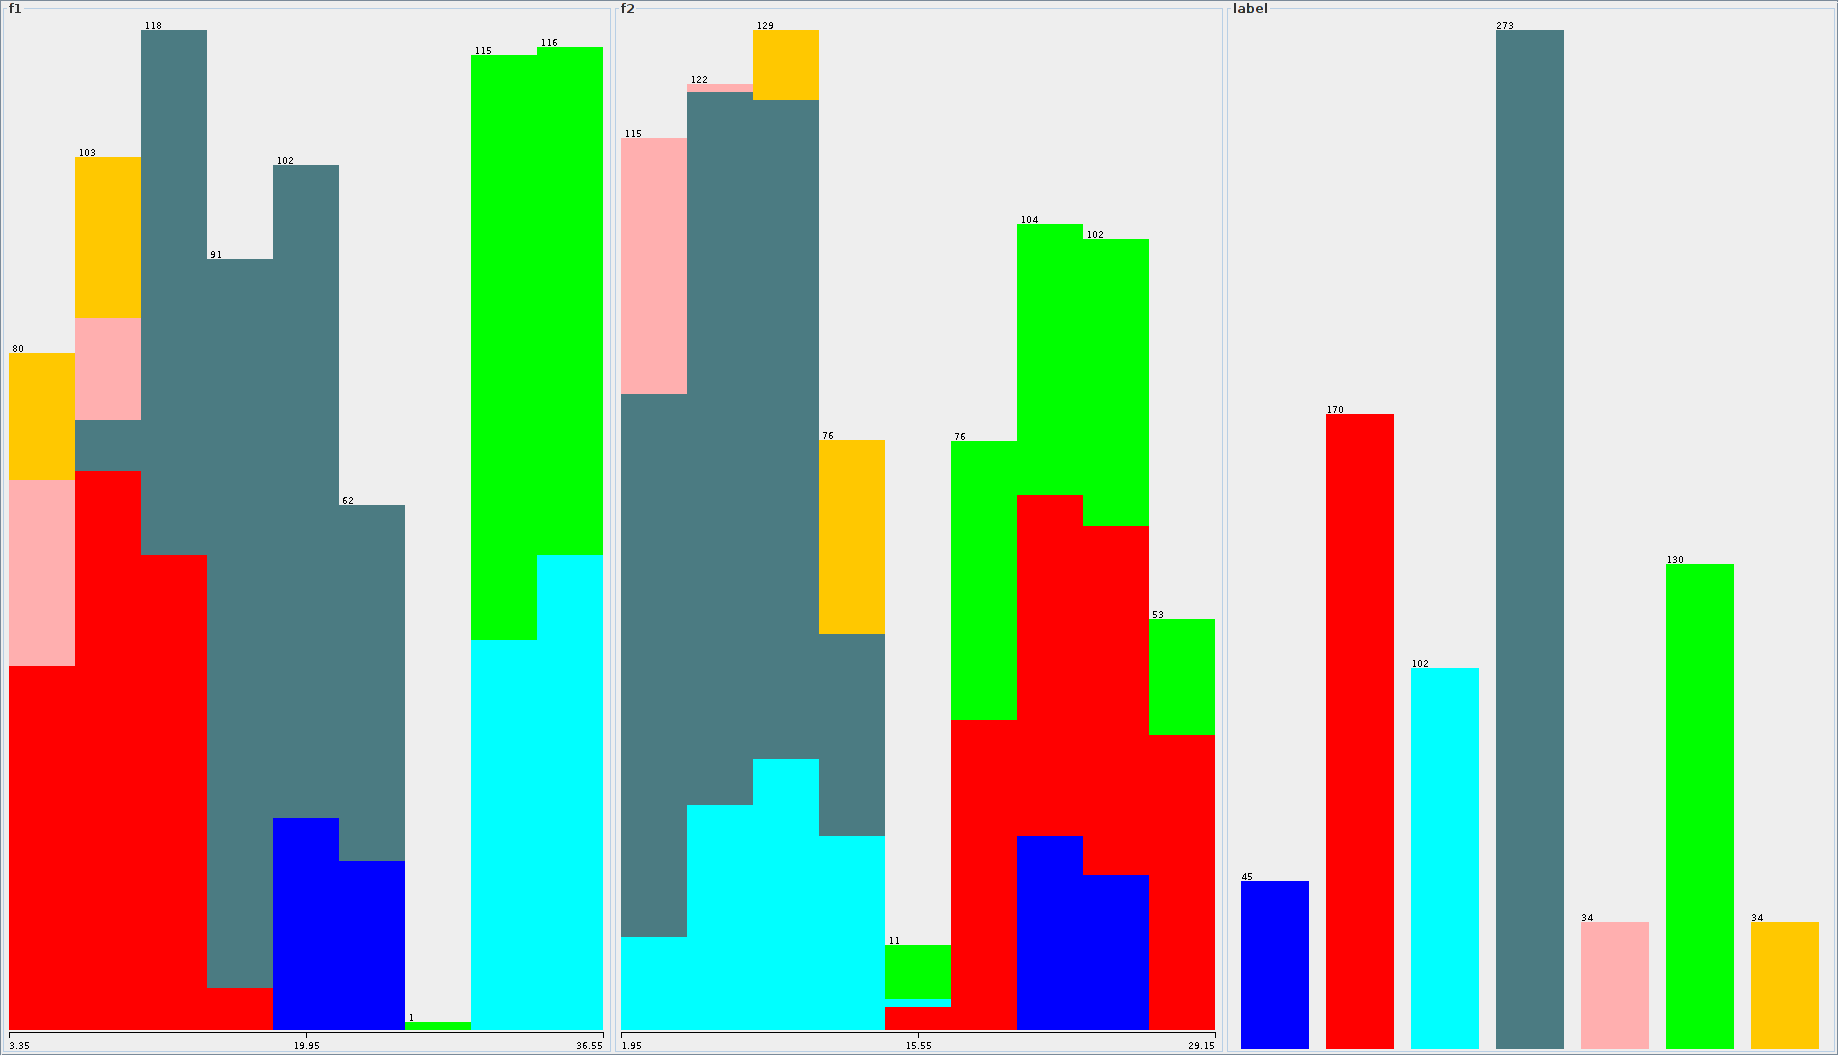
\includegraphics[width=0.7\textwidth]{Aggregation_4}\label{fig:f2}}
  \caption*{Classwise distribution of datapoints along features}
\end{figure}

As we can see below, the clusters are well enough space seperated  and hence K-means can converge to give optimum clusters that can be used for classification. The value of k has to chosen appropriately.

Clusters belonging to different classes have dense links between them. As a result, for very small $\epsilon$ and large MinPts, we probably would get bad results. But due to the interclass dense connection, it might cluster them together even for optimum $\epsilon$ and MinPts.

\begin{figure}[H]
  \centering
  \subfloat{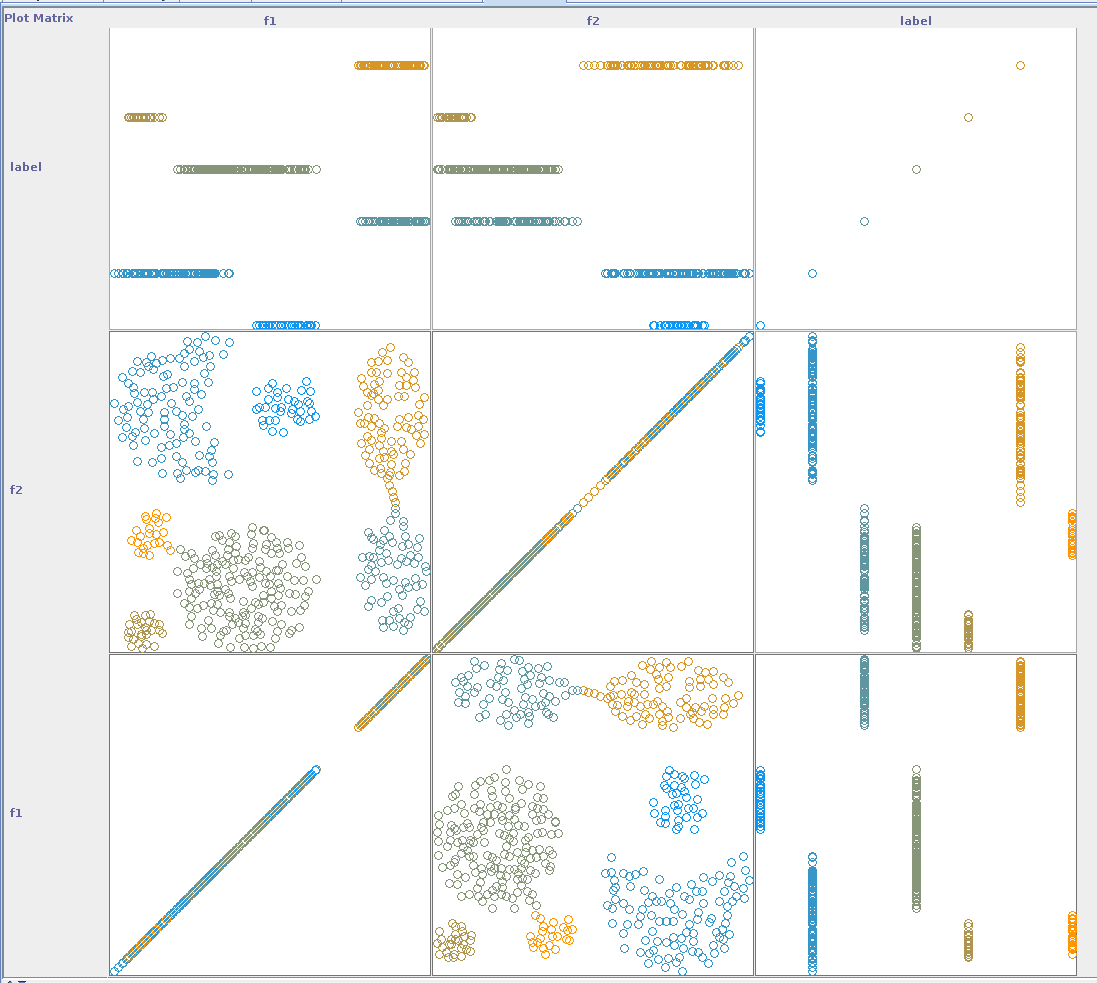
\includegraphics[width=0.6\textwidth]{Aggregation2}\label{fig:f1}}
  \hfill
  \subfloat{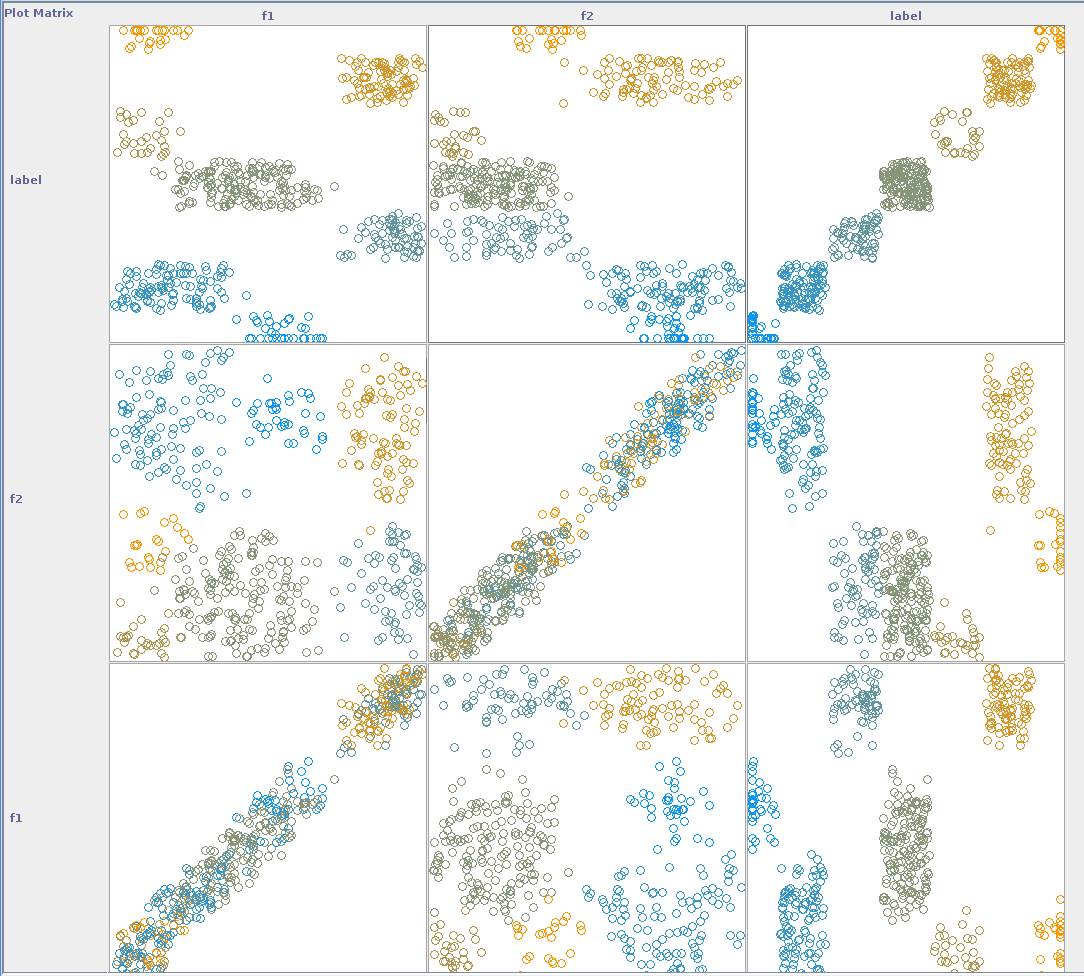
\includegraphics[width=0.6\textwidth]{Aggregation3}\label{fig:f2}}
  \caption*{Correlation Analysis}
\end{figure}

Single link has possibilities of merging the interconnected clusters. It might treat the interconnections as cluster and hence end up with non-optimum clustering.

Complete link might give us a very good clustering output in this case since the points in the same cluster are clustered together and complete link checks for the minimum distance between the farthest points in two clusters before merging them.

\subsubsection*{(ii)Compound}
\begin{figure}[H]
  \centering
  \subfloat{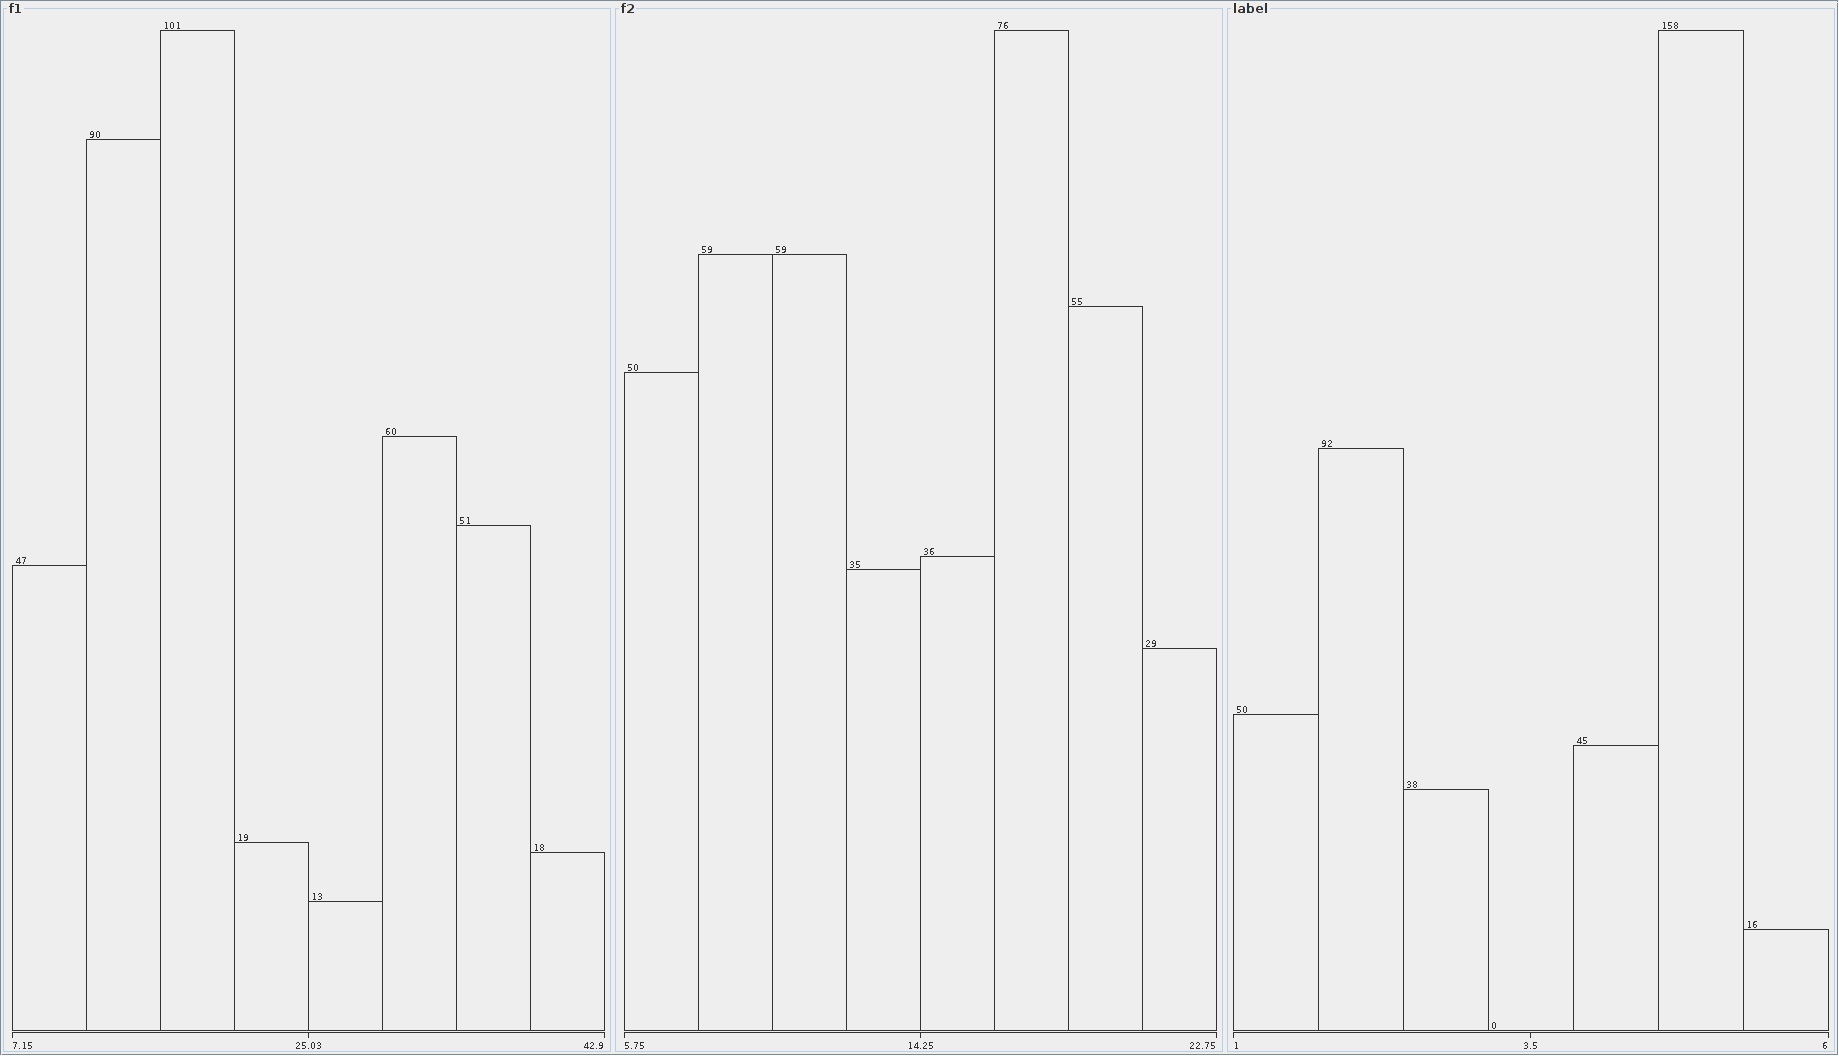
\includegraphics[width=0.8\textwidth]{Compound}\label{fig:f1}}
  \hfill
  \subfloat{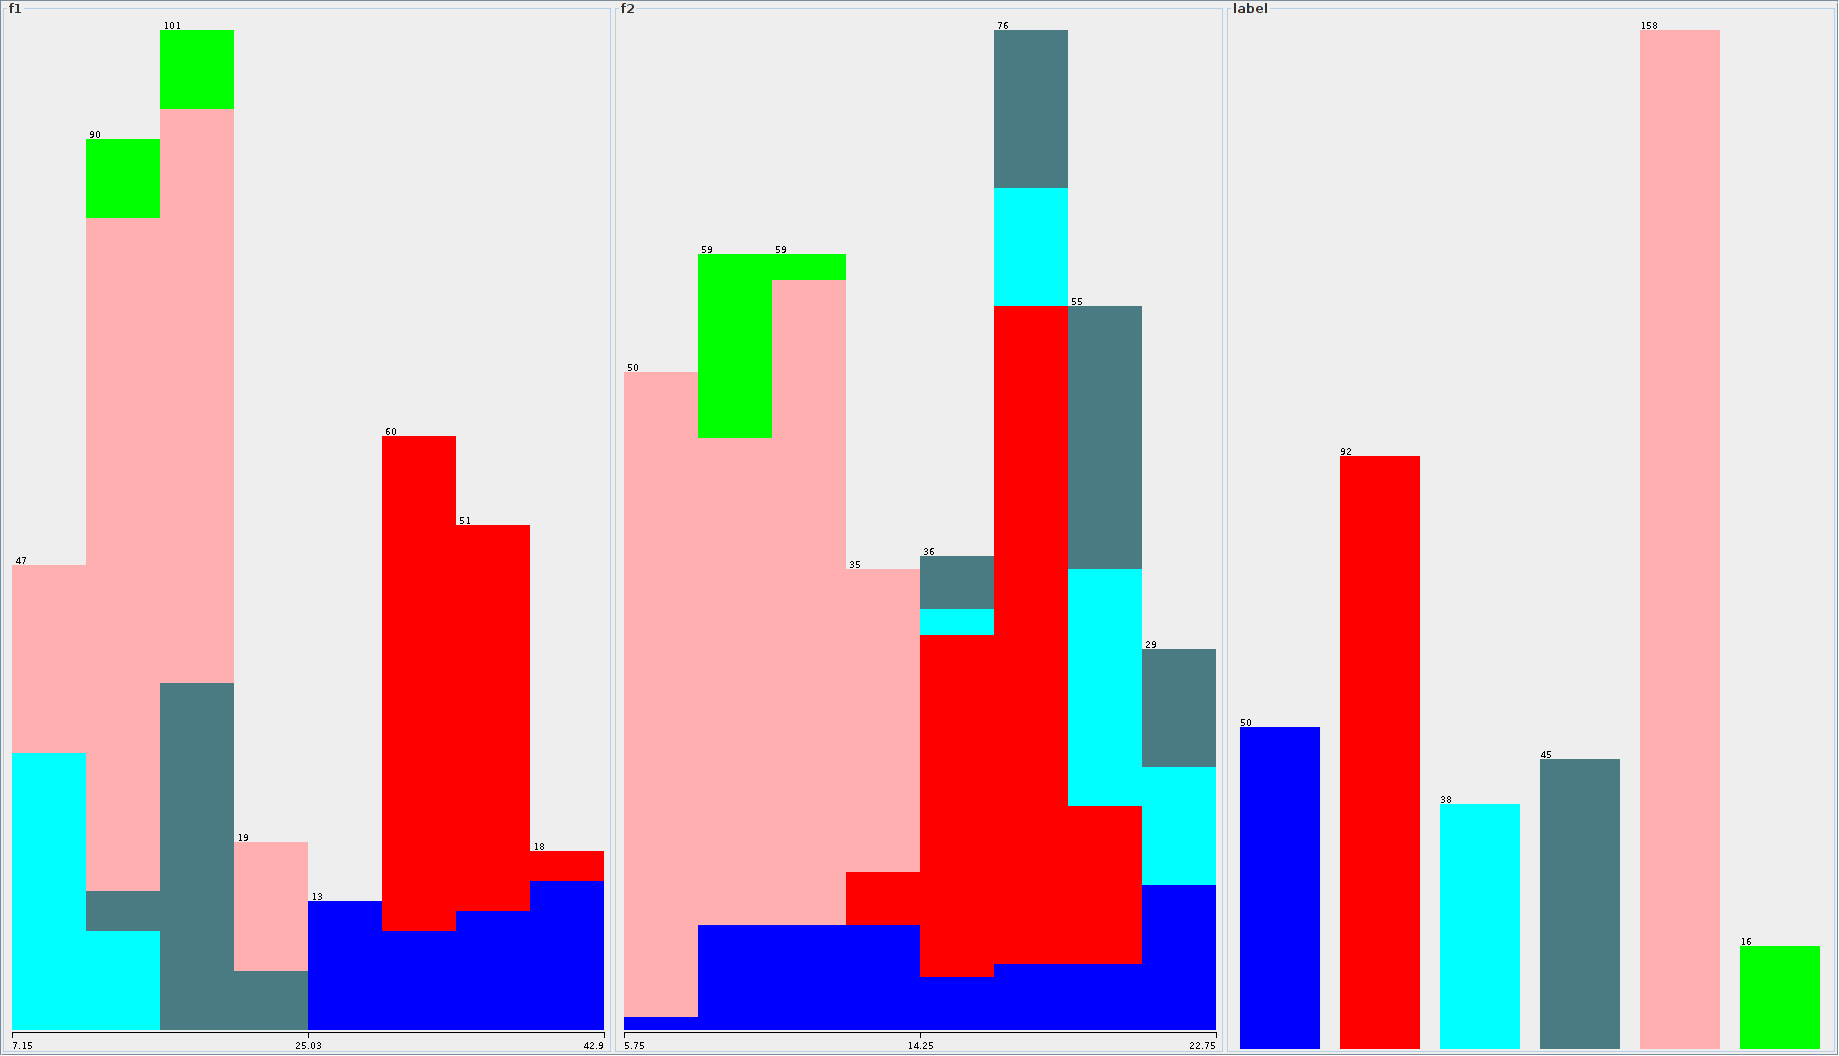
\includegraphics[width=0.8\textwidth]{Compound4}\label{fig:f2}}
  \caption*{Classwise distribution of datapoints along features}
\end{figure}

Since one class encircles another, K-means won't give us the best results since it is based on distance from centroids of points.

DBSCAN can identify the the classes having dense points such as with label 2,6,5,etc. But then it would fail in case of the datapoints in less dense classes. For higher value of $\epsilon$, it would end up merging classes.

Single link might converge to a similar situation as DBSCAN. This is because of the encirclement of one class by another and due to the difference in class densities.

Complete Link might give us a good solution since it merges the clusters having minimum distance between the farthest datapoint in each cluster. Hence, we might reach a solution where in, by merging a few clusters, we can find a very good class seperation.

\begin{figure}[H]
  \centering
  \subfloat{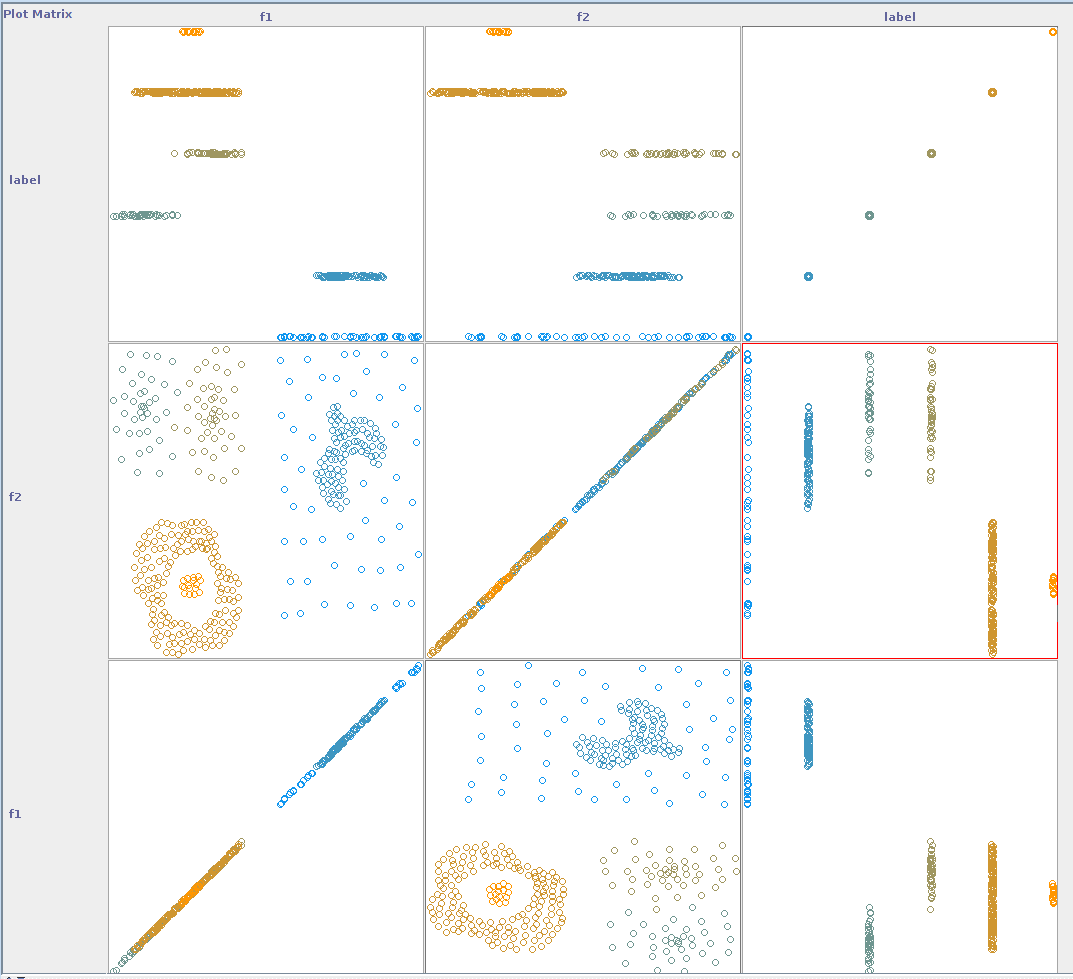
\includegraphics[width=0.7\textwidth]{Compound2}\label{fig:f1}}
  \hfill
  \subfloat{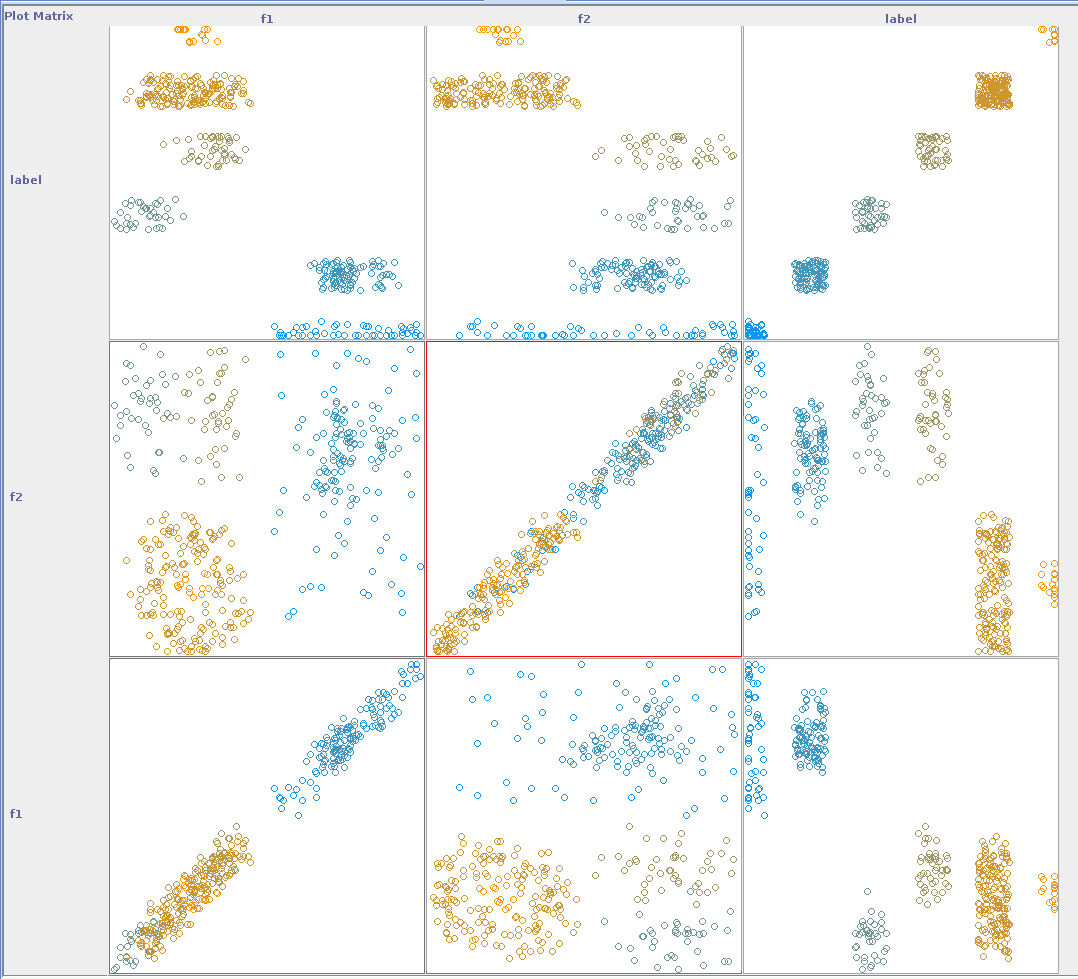
\includegraphics[width=0.7\textwidth]{Compound3}\label{fig:f2}}
  \caption*{Correlation Analysis}
\end{figure}


\subsubsection*{(iii)D31}
\begin{figure}[H]
  \centering
  \subfloat{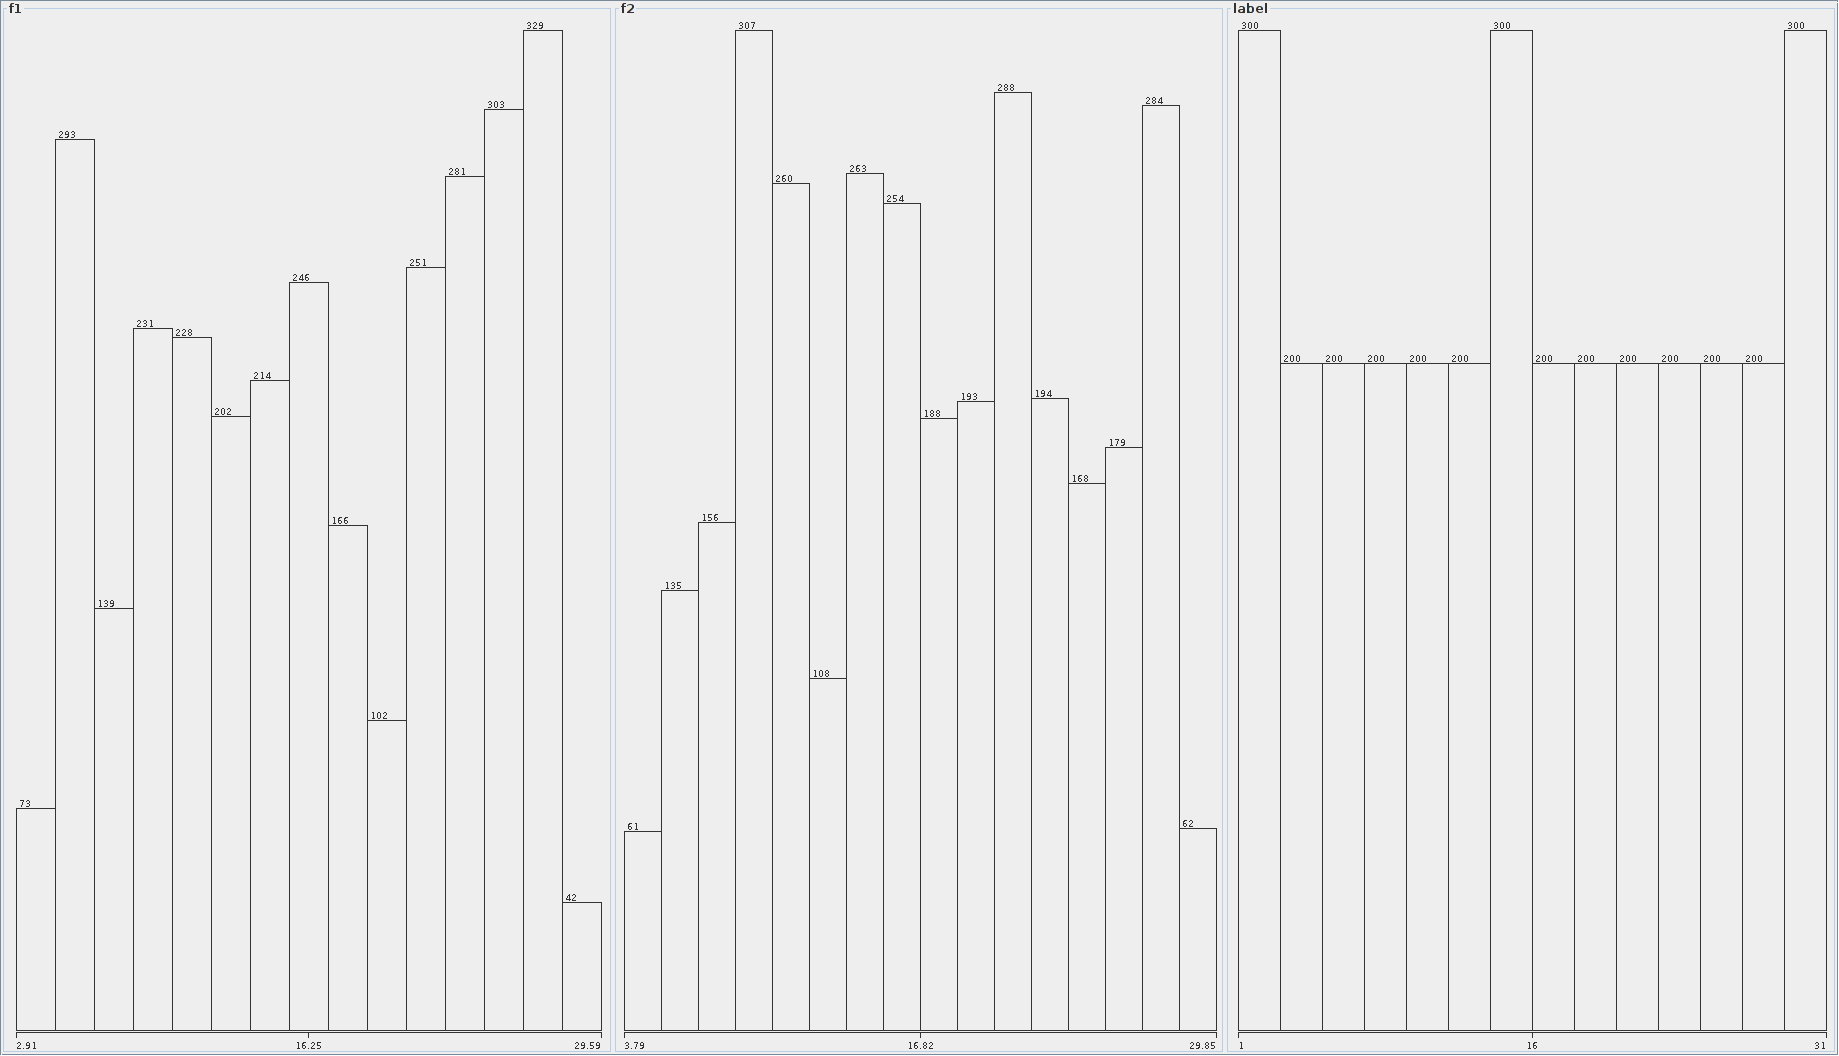
\includegraphics[width=0.8\textwidth]{D31}\label{fig:f1}}
  \hfill
  \subfloat{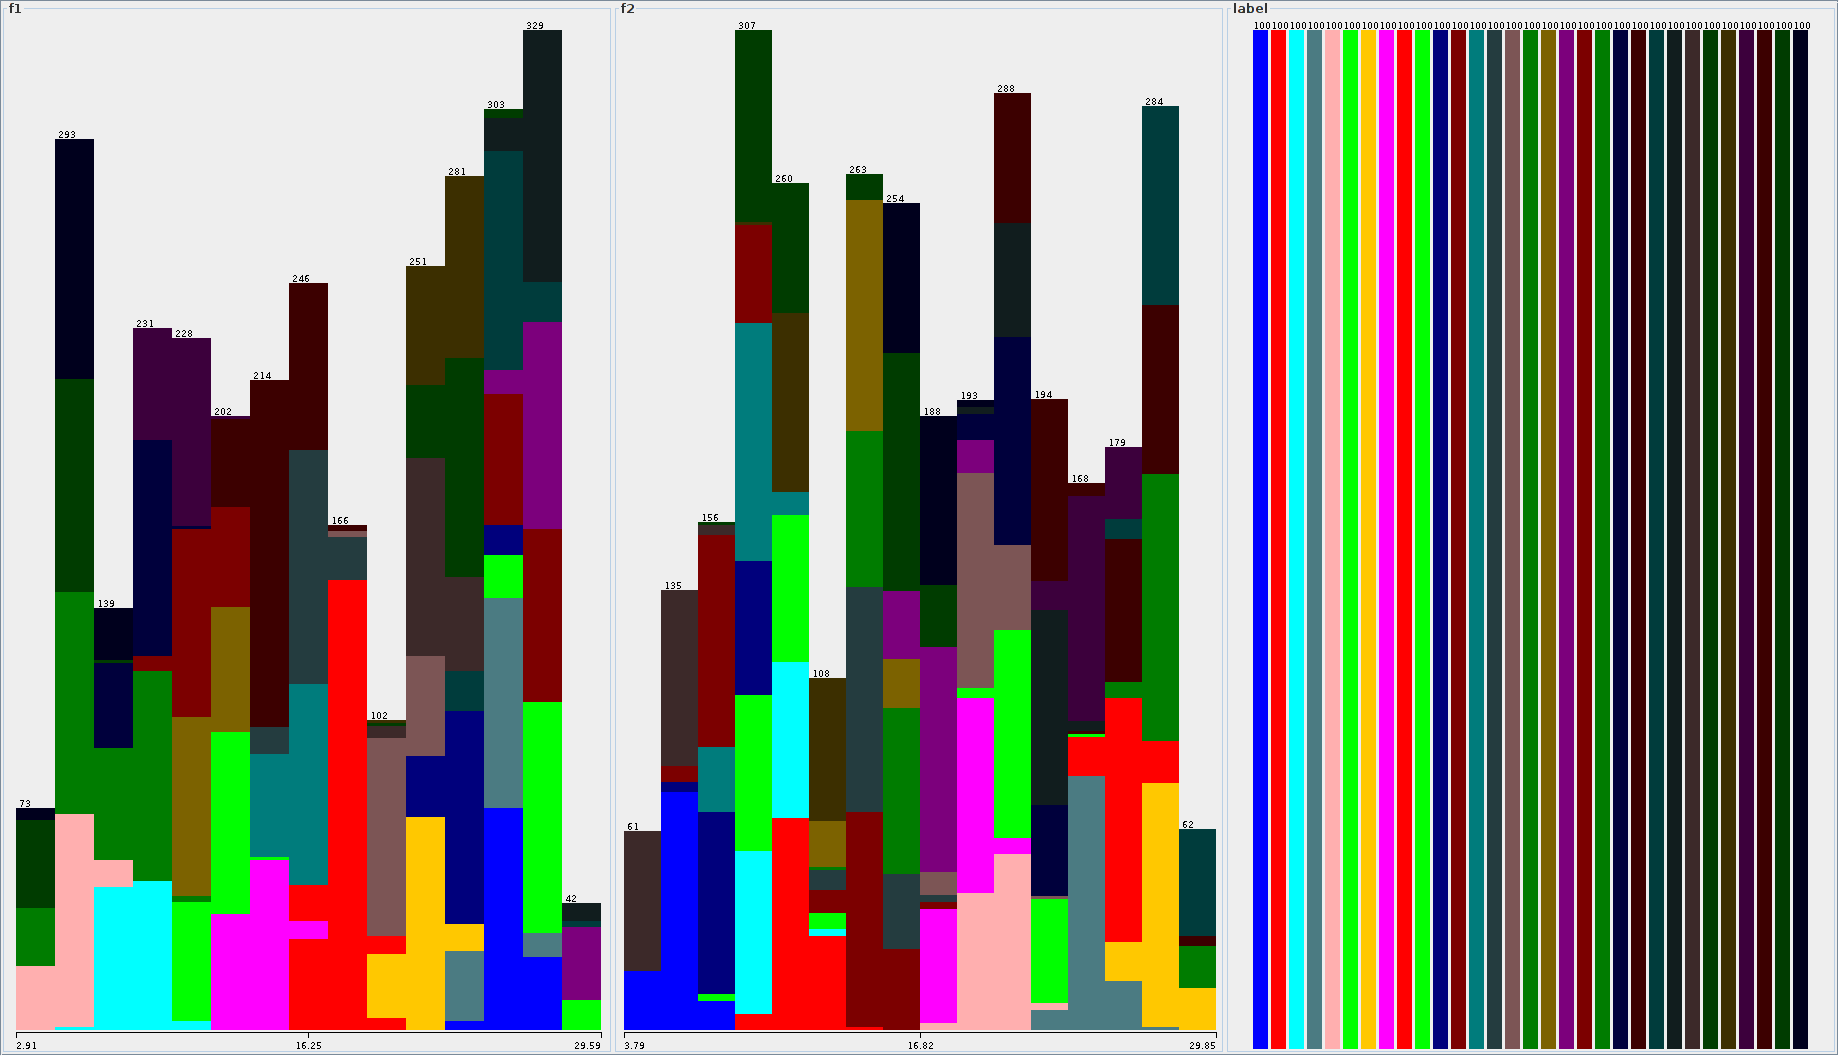
\includegraphics[width=0.8\textwidth]{D31_4}\label{fig:f2}}
  \caption*{Classwise distribution of datapoints along features}
\end{figure}

Since the datapoints are well seperated with sufficient between class variance and small in-class variance, K-means can give us very good clustering results.

Since the points belonging to the same class are densely clusterd together, DBSCAN can give us very good results by appropriately choosing $\epsilon$ and MinPts.

Since the points belonging to the same class are densely clusterd together(less distance between points), Single link hierarchial clustering can give us good results, as it checks for the distance between the nearest datapints in two clusters before merging them.

Complete Link might not give us a good solution since it merges the clusters having minimum distance between the farthest datapoint in each cluster. Hence, we might reach a solution where in, set of datapoints belonging to one class gets merged with another.

\begin{figure}[H]
  \centering
  \subfloat{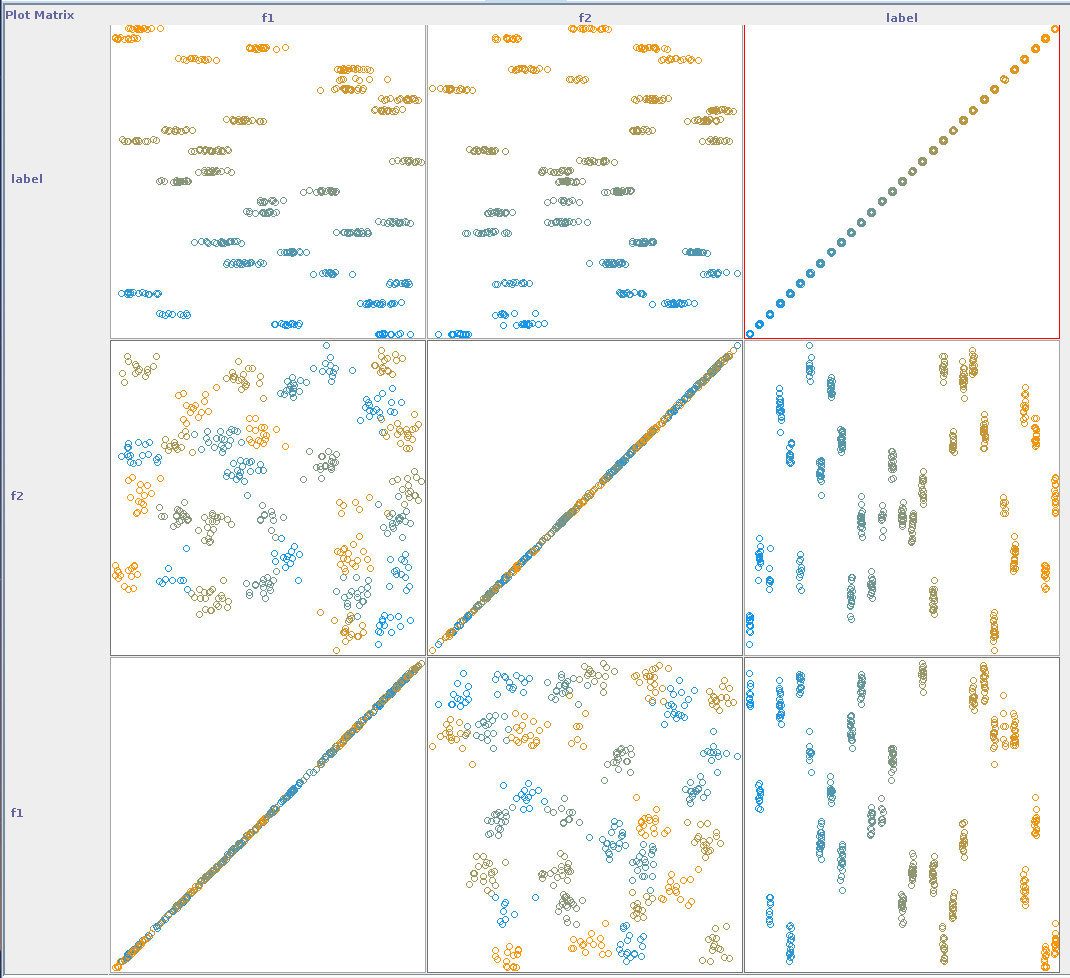
\includegraphics[width=0.7\textwidth]{D31_2}\label{fig:f1}}
  \hfill
  \subfloat{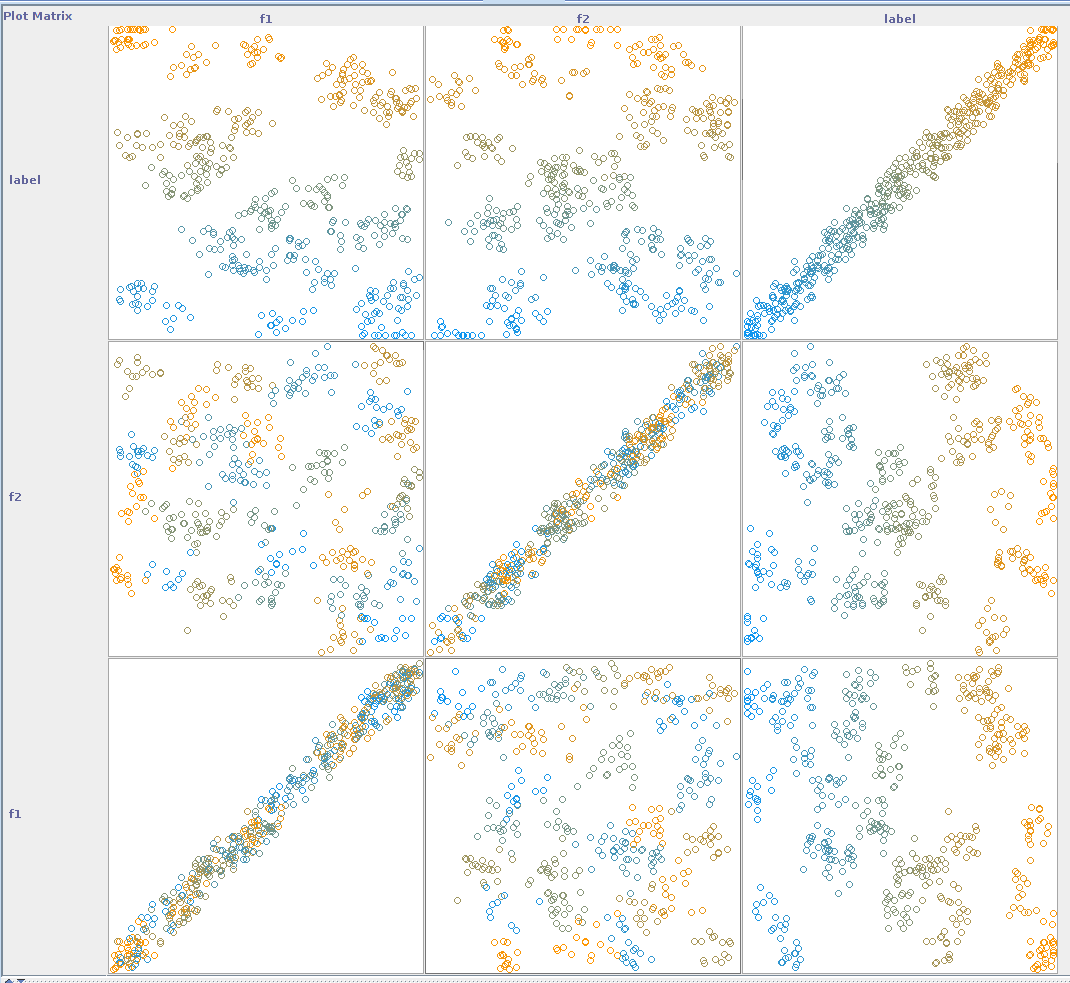
\includegraphics[width=0.7\textwidth]{D31_3}\label{fig:f2}}
  \caption*{Correlation Analysis}
\end{figure}


\subsubsection*{(iv)Flames}
\begin{figure}[H]
  \centering
  \subfloat{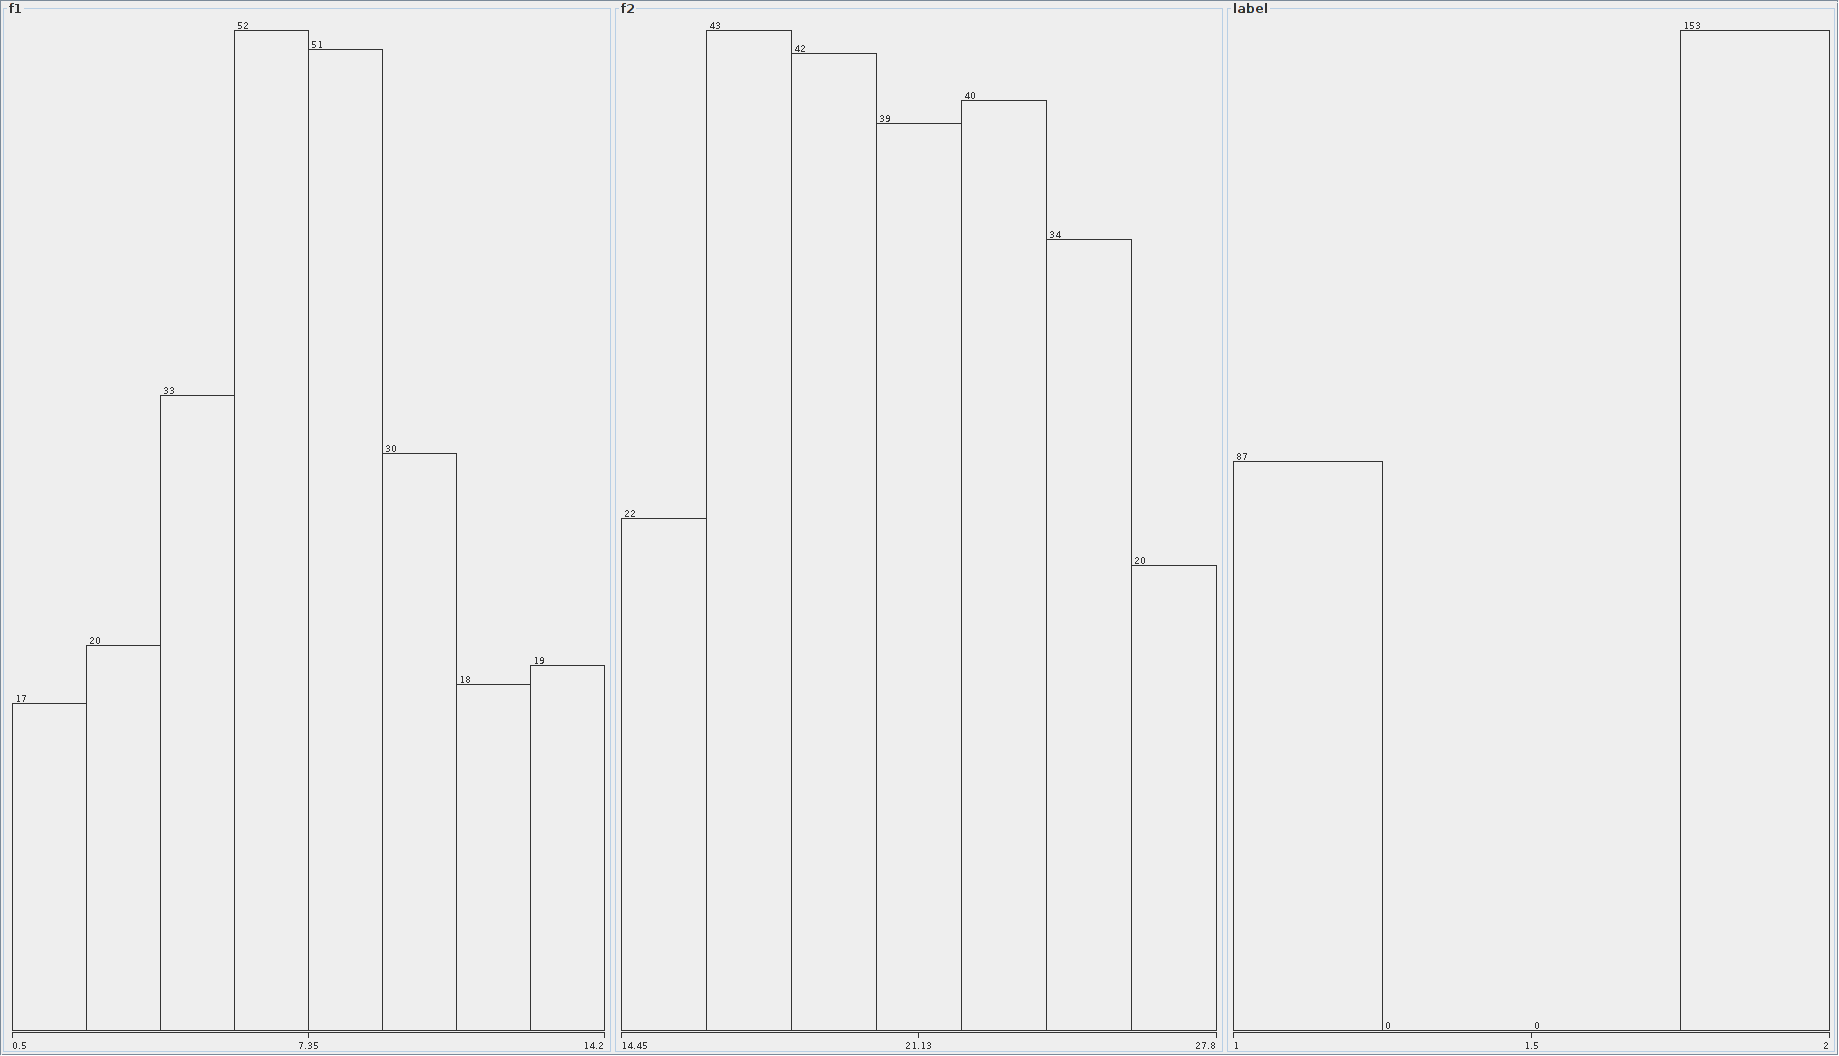
\includegraphics[width=0.8\textwidth]{Flames}\label{fig:f1}}
  \hfill
  \subfloat{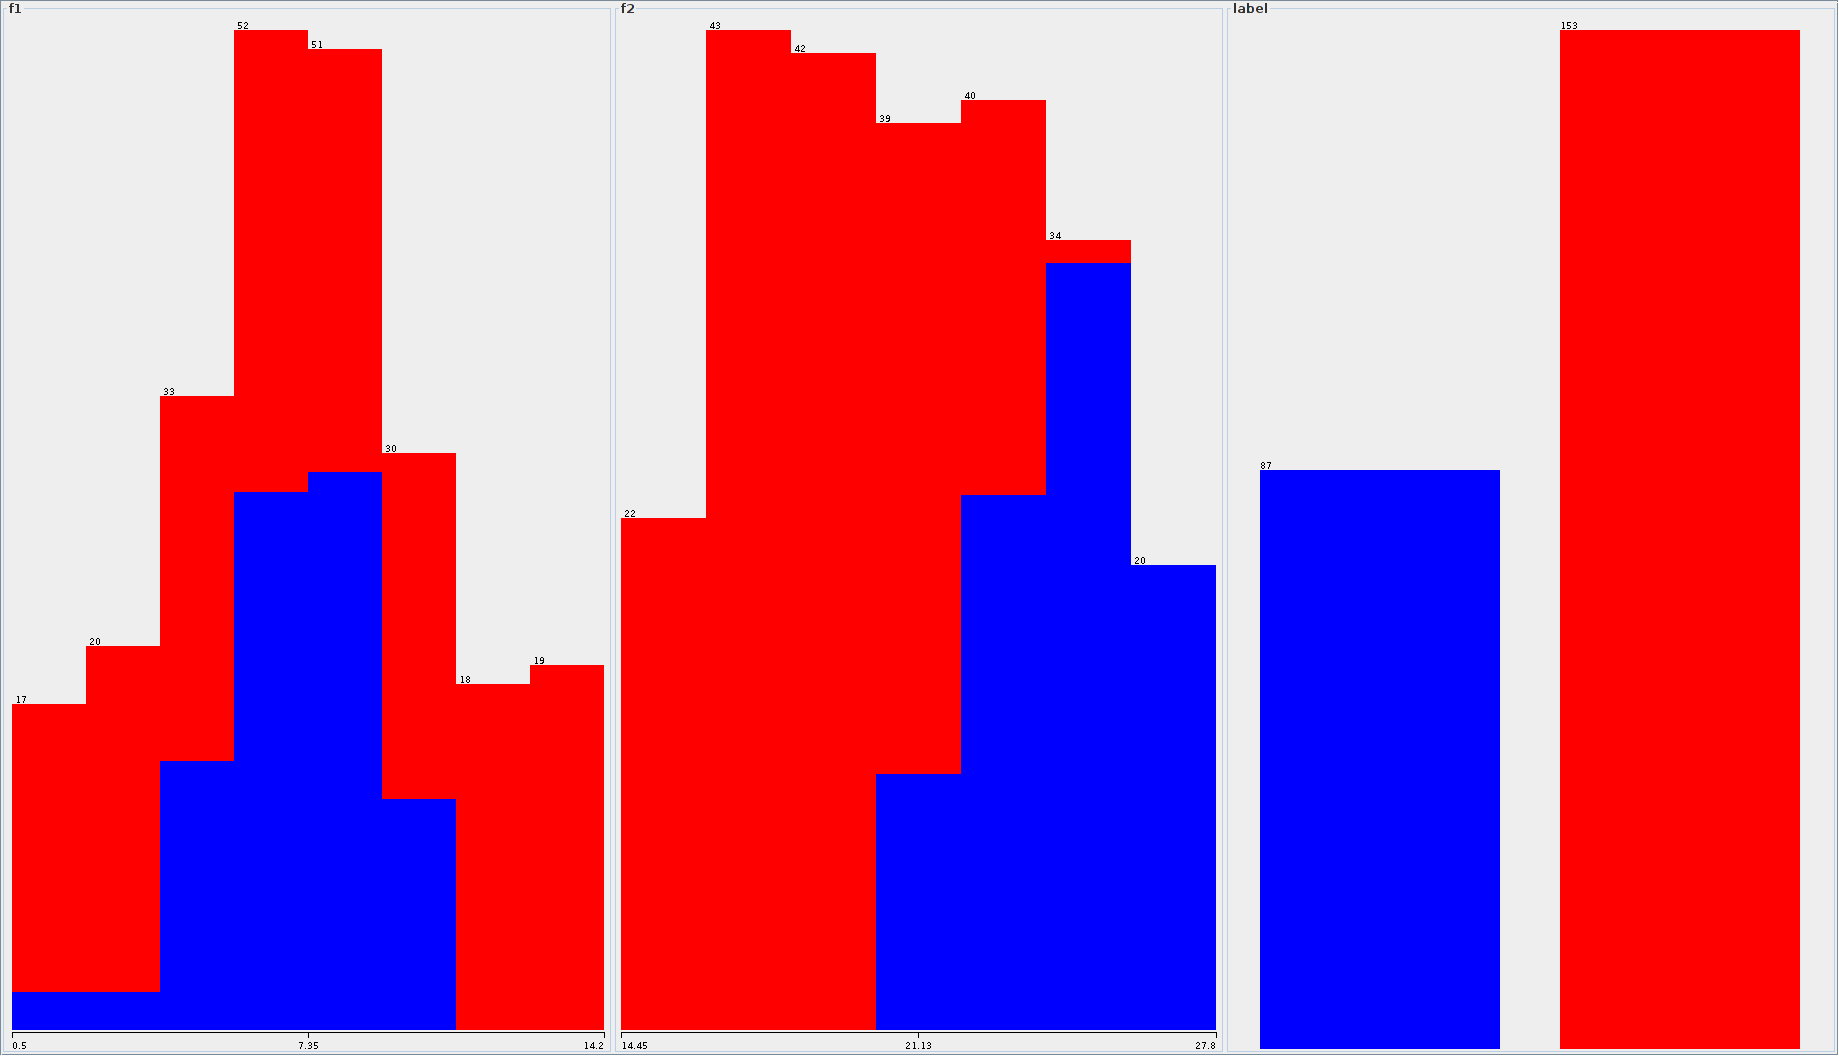
\includegraphics[width=0.8\textwidth]{Flames4}\label{fig:f2}}
  \caption*{Classwise distribution of datapoints along features}
\end{figure}

K-Means wont give us the optimum solution since one class partially encircles the other. Hence, K-means ends up misclassifying points.

DBSCAN will work really well for the given dataset since the points belonging to the same cluster are uniformly distributed(almost same density) and the density of the two classes are also nearly the same. Hence we get optimum clustering.

Since the points belonging to the same class are densely clusterd together(less distance between points), Single link hierarchial clustering can give us good results, as it checks for the distance between the nearest datapints in two clusters before merging them.

Complete Link might not give us a good solution since it merges the clusters having minimum distance between the farthest datapoint in each cluster. Hence, we might reach a solution where in, set of datapoints belonging to one class gets merged with another. This is because the outer class is elongated and hence, Complete link might start merging a part of the other class(like a disk) with the existing clusters found using complete link while forming merges.

\begin{figure}[H]
  \centering
  \subfloat{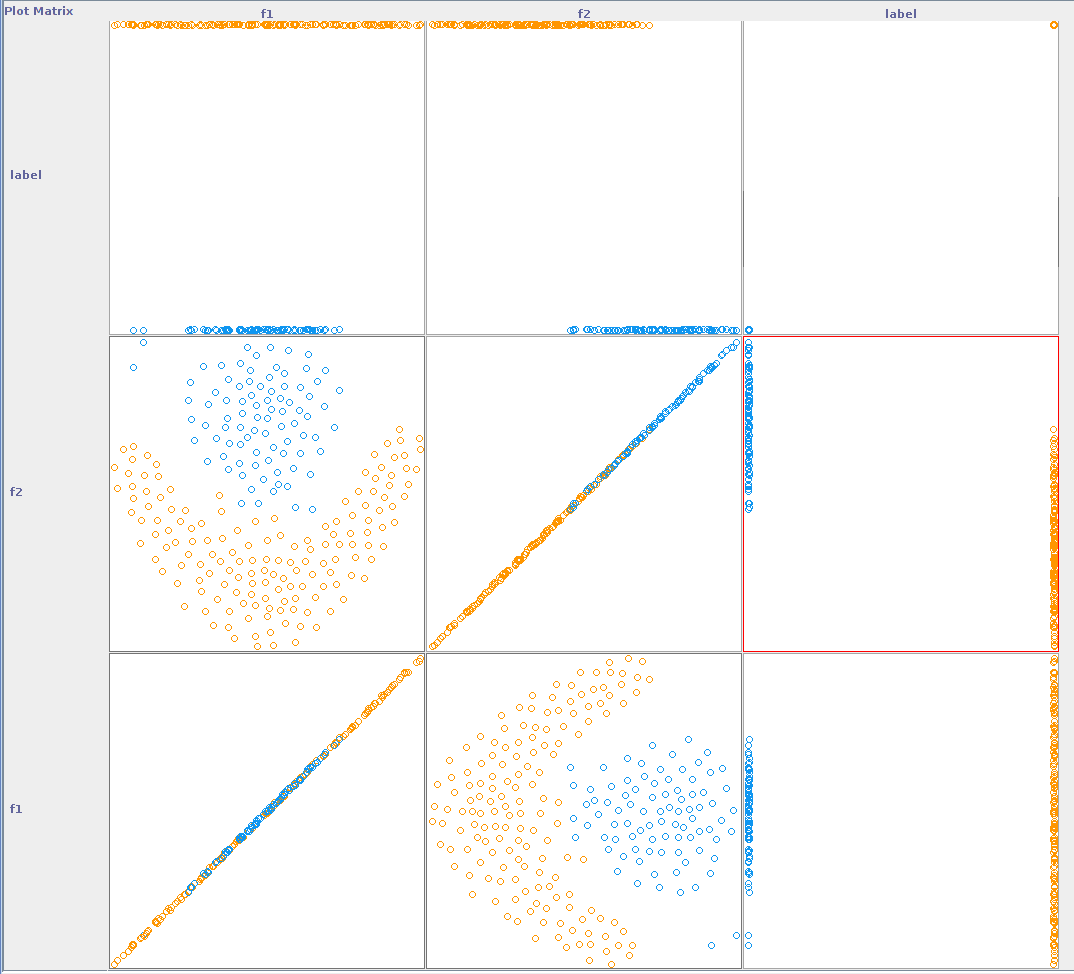
\includegraphics[width=0.65\textwidth]{Flames2}\label{fig:f1}}
  \hfill
  \subfloat{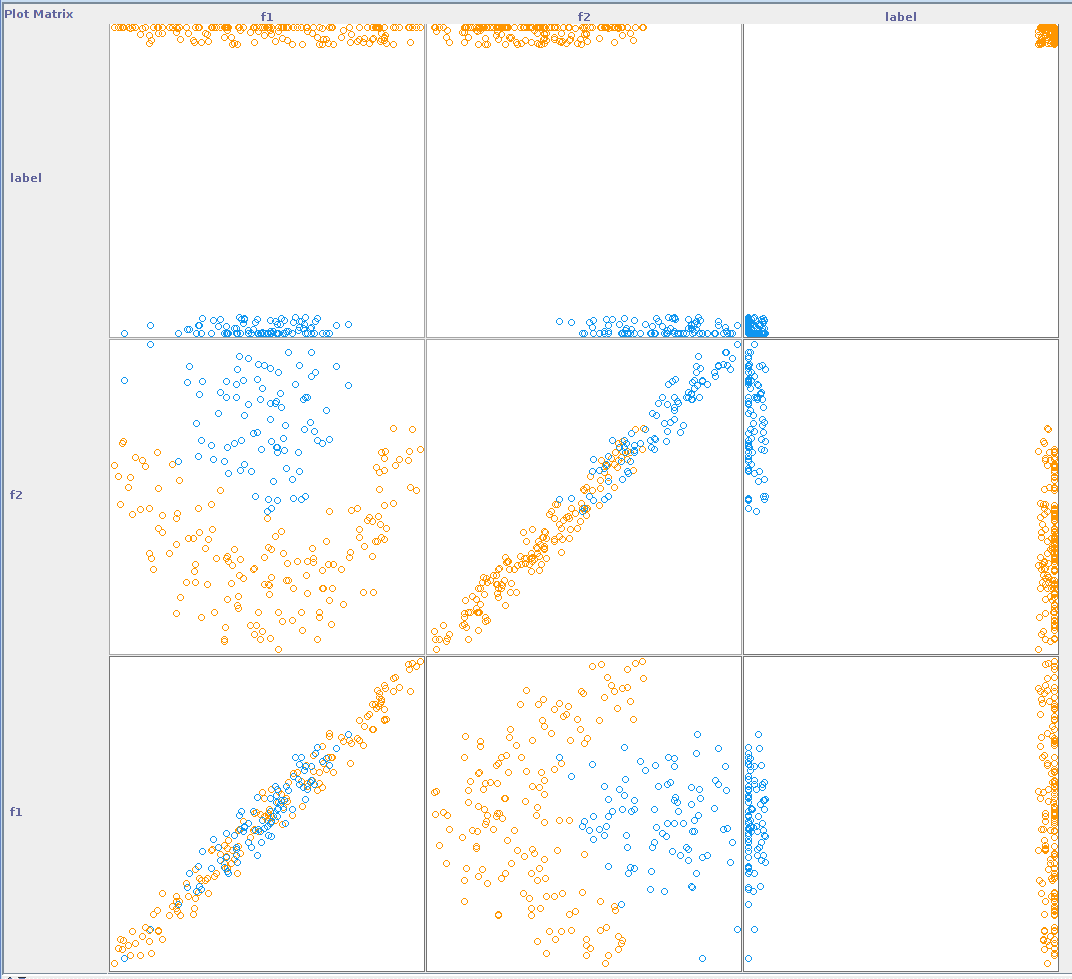
\includegraphics[width=0.6\textwidth]{Flames3}\label{fig:f2}}
  \caption*{Correlation Analysis}
\end{figure}

\subsubsection*{(v)Jain}
\begin{figure}[H]
  \centering
  \subfloat{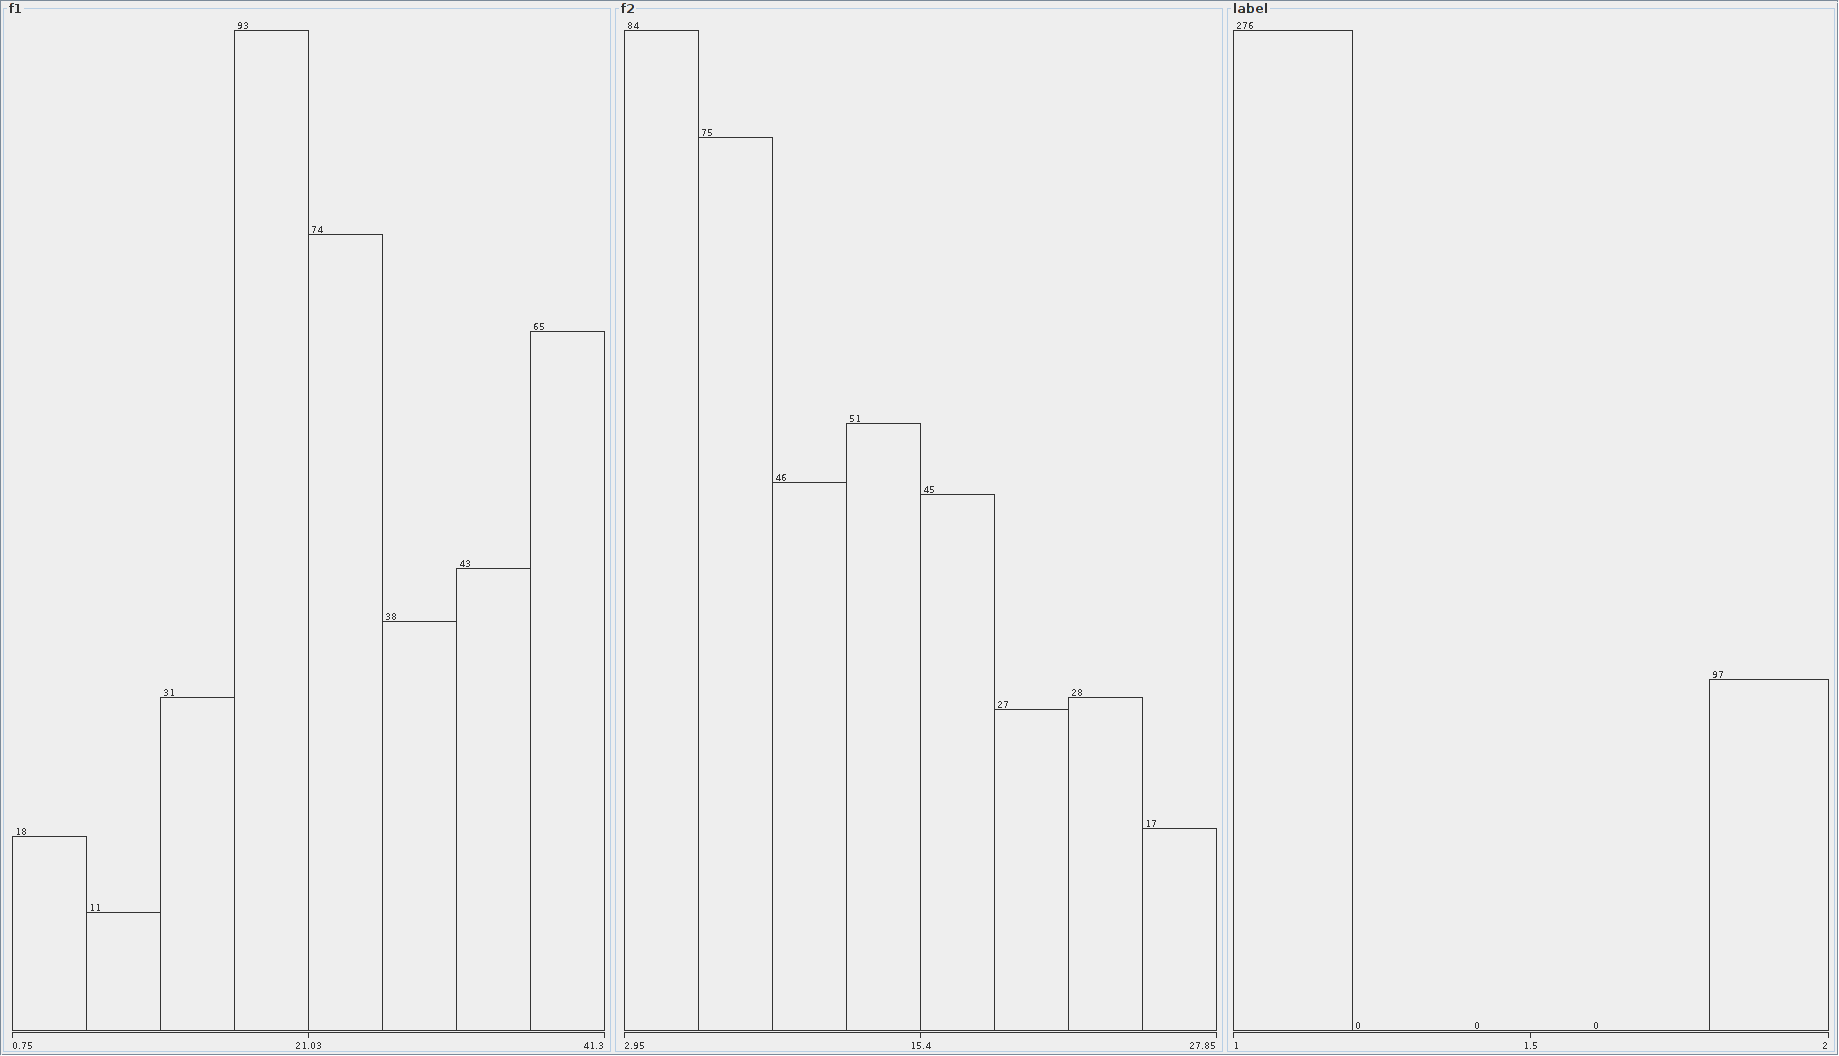
\includegraphics[width=0.8\textwidth]{Jain}\label{fig:f1}}
  \hfill
  \subfloat{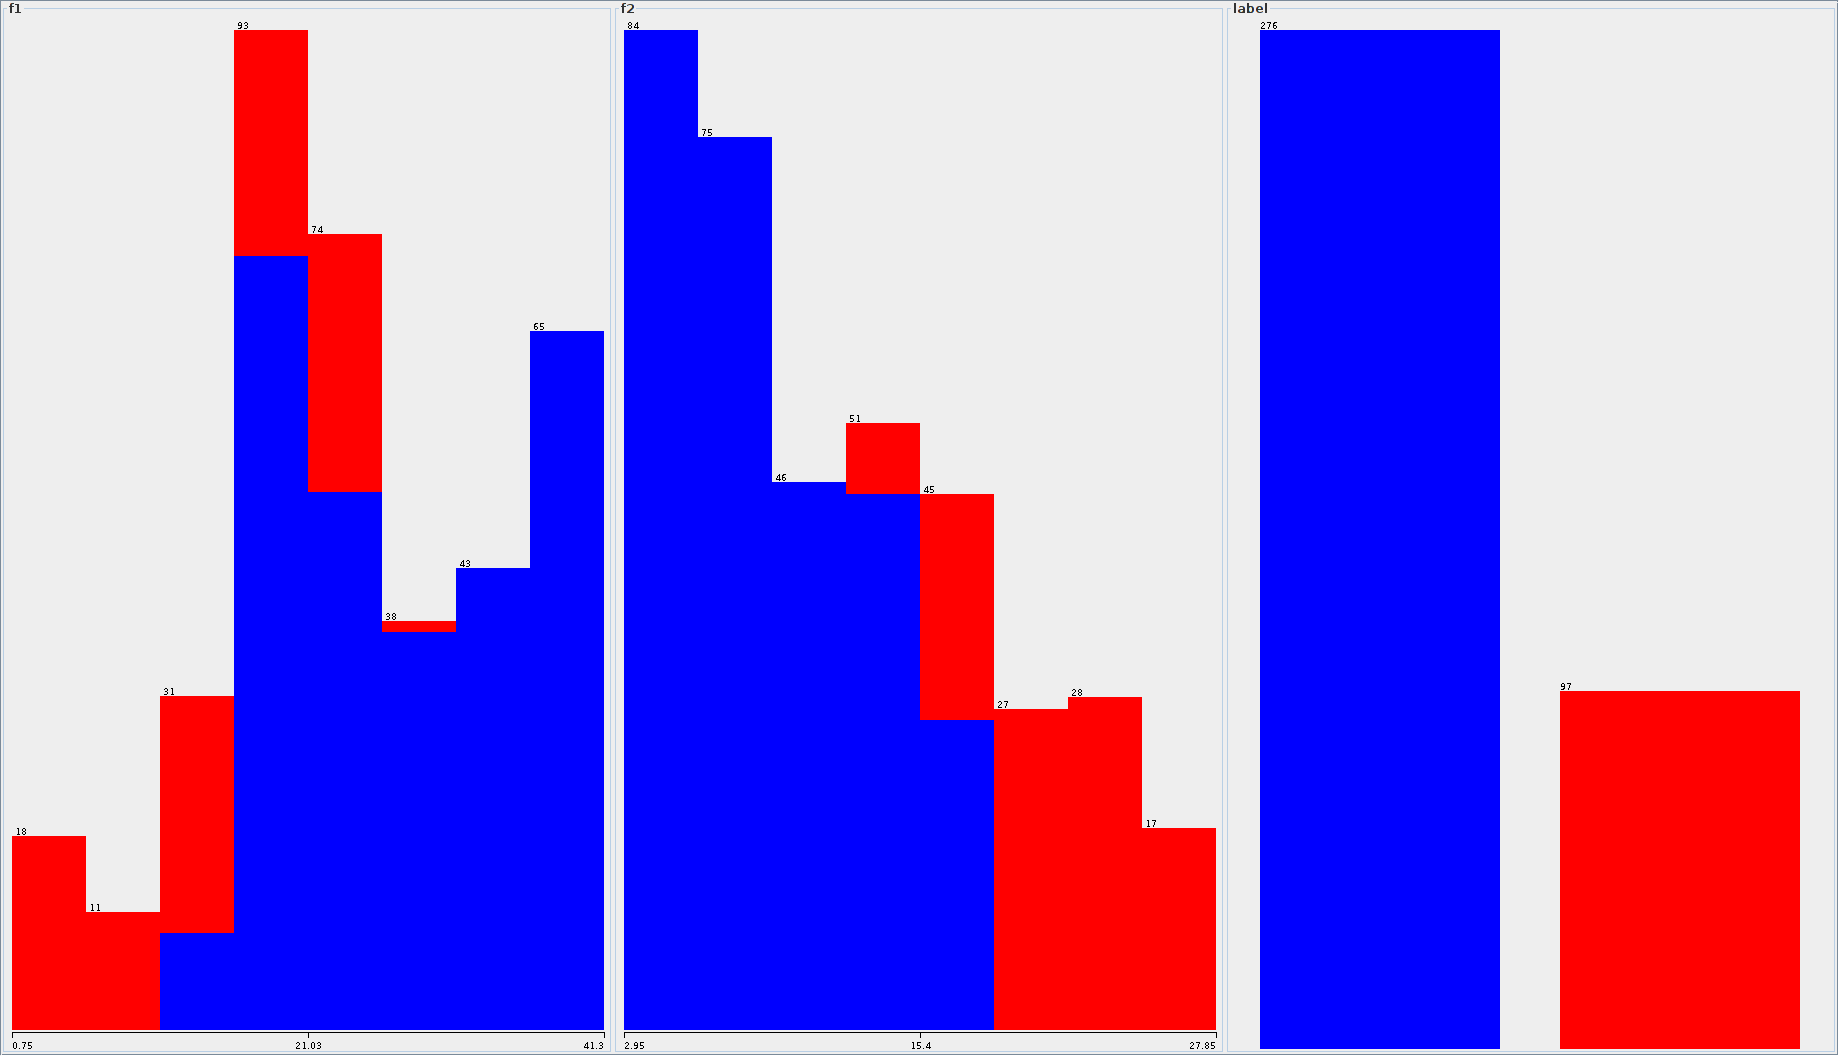
\includegraphics[width=0.8\textwidth]{Jain4}\label{fig:f2}}
  \caption*{Classwise distribution of datapoints along features}
\end{figure}

Due to partial encirclement, K-means would misclassify some datapoints adn it would find a cluster seperation that is nearly a straight line, since it works on the principle of minimising the cluster centroids.

As the density within a class is almost uniform, DBSCAN may find optimum clusters, but it would depend on the relative densities between the classes as well. It may happen that a fraction of class yellow is treated as noise. 

Since the points belonging to the same class are densely clusterd together(less distance between points), Single link hierarchial clustering can give us good results, as it checks for the distance between the nearest datapints in two clusters before merging them. 

Complete Link might not give us a good solution since it merges the clusters having minimum distance between the farthest datapoint in each cluster. Hence, we might reach a solution where in, set of datapoints belonging to one class gets merged with another. This is because the classes are elongated and partially encircling and hence, Complete link might start merging a part of the other class with the existing clusters found using complete link while forming merges. If there are cluster points in yellow closer to blue, then they will get misclassified.


\begin{figure}[H]
  \centering
  \subfloat{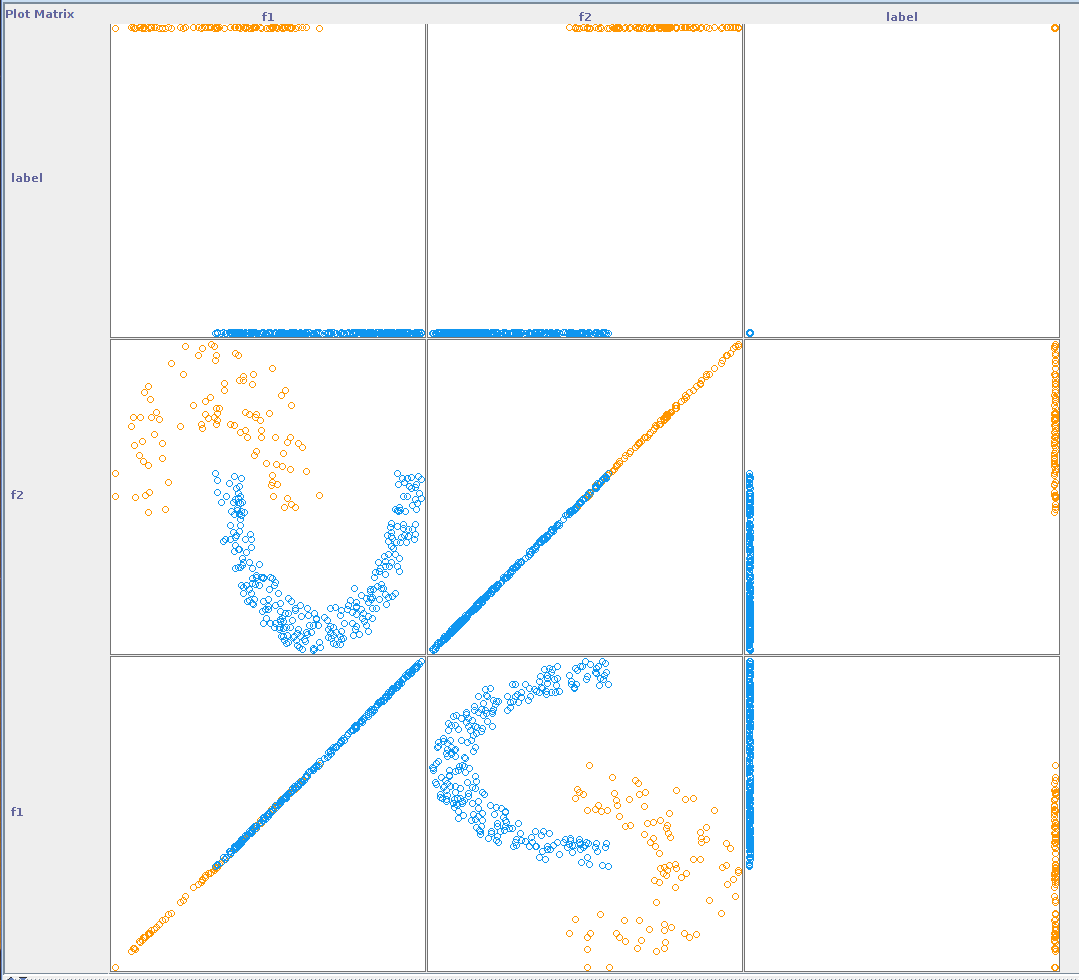
\includegraphics[width=0.6\textwidth]{Jain2}\label{fig:f1}}
  \hfill
  \subfloat{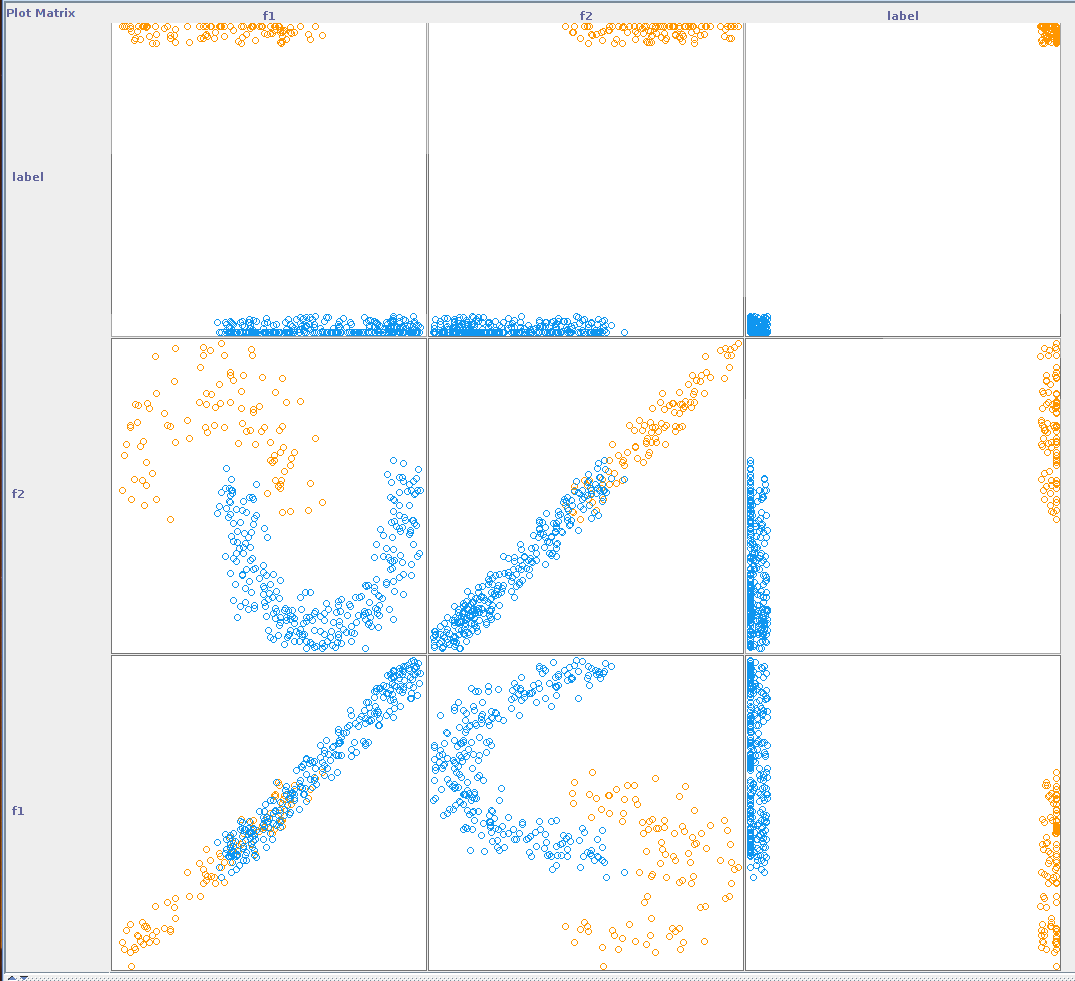
\includegraphics[width=0.6\textwidth]{Jain3}\label{fig:f2}}
  \caption*{Correlation Analysis}
\end{figure}


\subsubsection*{(vi)Path-based}
\begin{figure}[H]
  \centering
  \subfloat{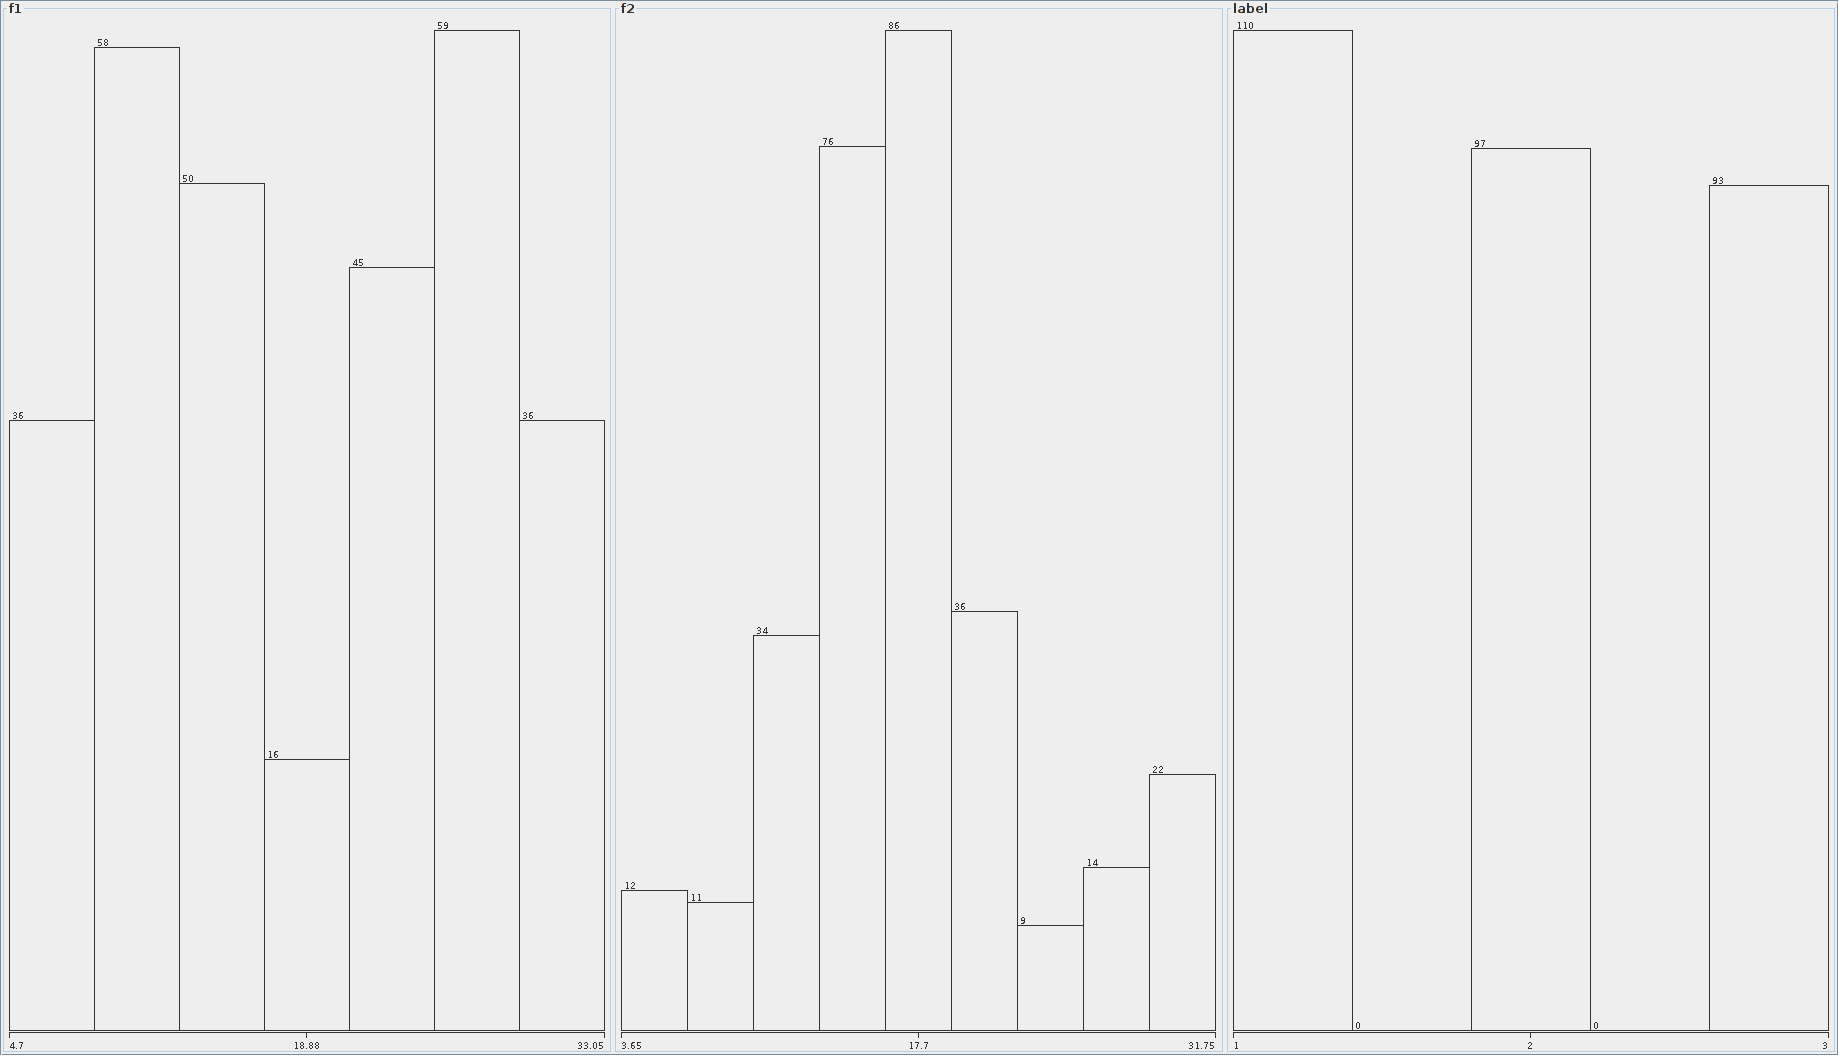
\includegraphics[width=0.8\textwidth]{Path-based}\label{fig:f1}}
  \hfill
  \subfloat{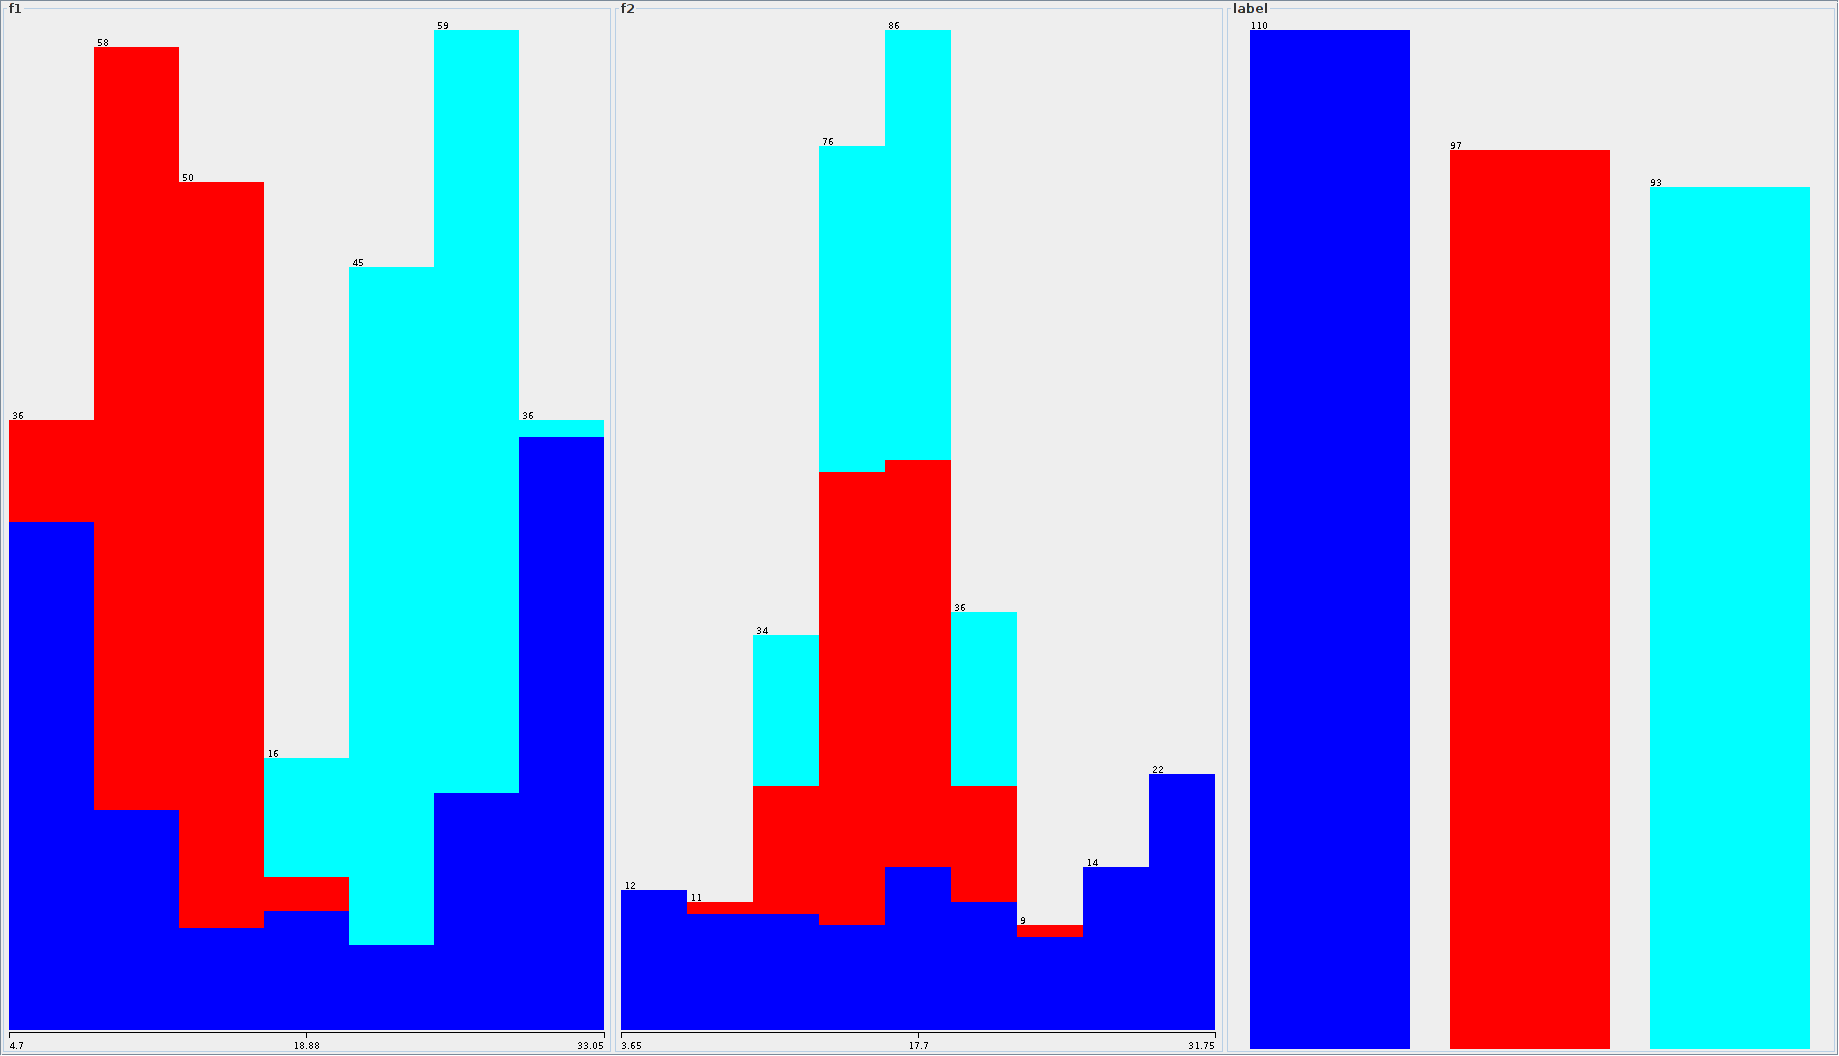
\includegraphics[width=0.8\textwidth]{Path-based4}\label{fig:f2}}
  \caption*{Classwise distribution of datapoints along features}
\end{figure}

K-means would fail in the identification of 3 clusters, as one cluster is encircling the other two. Hence two classes can be correctly identified but a large fraction of the blus class gets misclassified.

As the density within a class is almost uniform, DBSCAN can find optimum clusters, but it would depend on the relative densities between the classes as well. It may happen that a fraction of class yellow or green are treated as noise. But by right choice of $\epsilon$ and MinPts, we may be able to find the optimum clustering.

Since the points belonging to the same class are densely clusterd together(less distance between points), Single link hierarchial clustering may give us good results, as it checks for the distance between the nearest datapints in two clusters before merging them. But it might misclassify the datapoints belonging to different classes that are close to one another.

Complete Link won't give us a good solution since it merges the clusters having minimum distance between the farthest datapoint in each cluster. Hence, we might reach a solution where in, set of datapoints belonging to one class gets merged with another. This is because the blue classe is elongated and partially encircling the other two classes and hence, Complete link might start merging a part of the other class with the existing clusters found using complete link while forming merges. 

\begin{figure}[H]
  \centering
  \subfloat{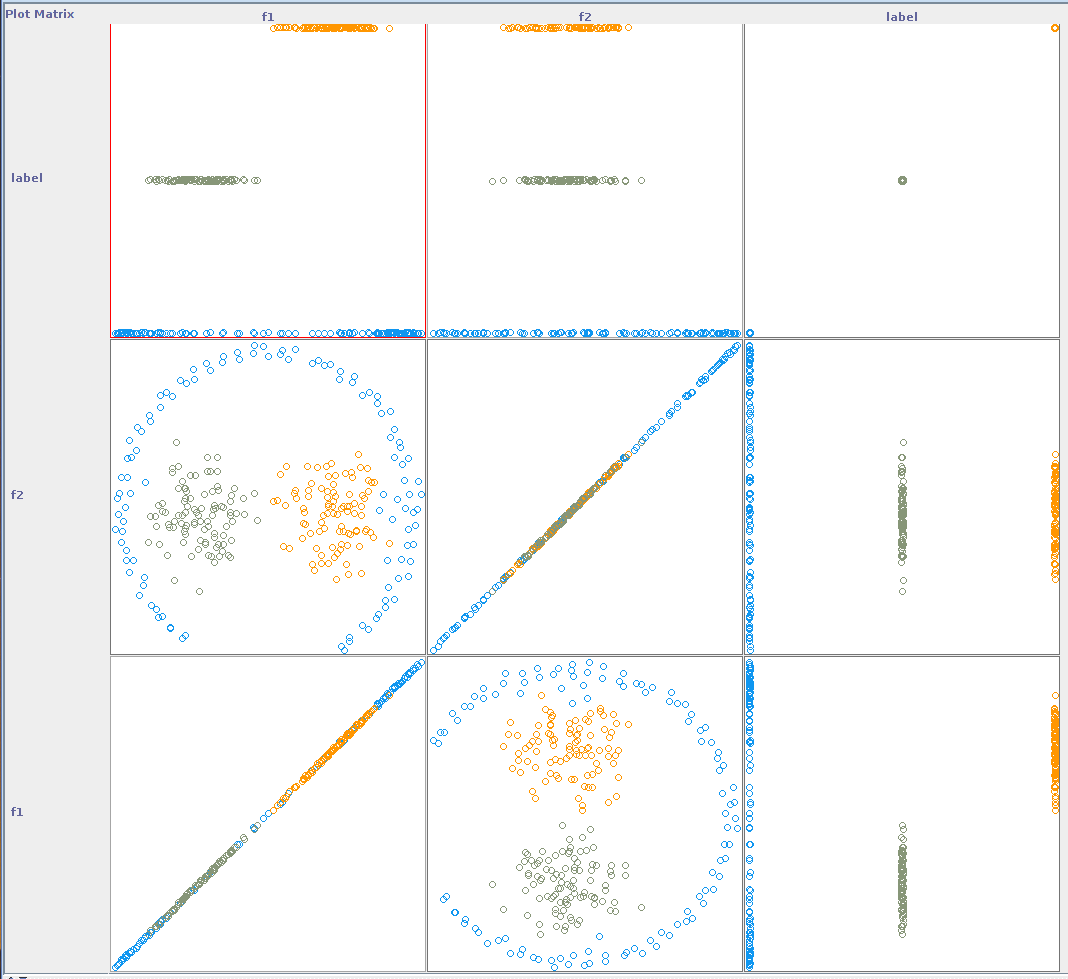
\includegraphics[width=0.6\textwidth]{Path-based2}\label{fig:f1}}
  \hfill
  \subfloat{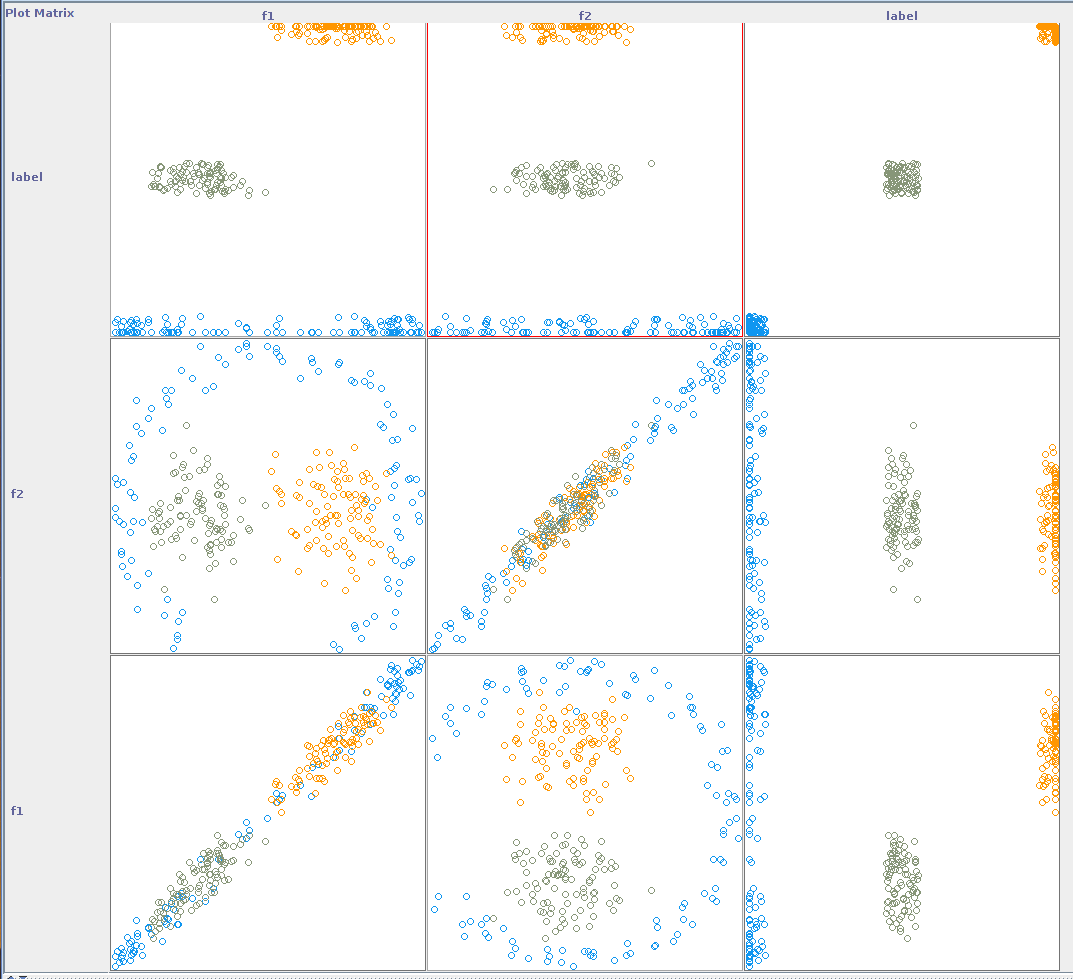
\includegraphics[width=0.55\textwidth]{Path-based3}\label{fig:f2}}
  \caption*{Correlation Analysis}
\end{figure}

\subsubsection*{(vii)R15}
\begin{figure}[H]
  \centering
  \subfloat{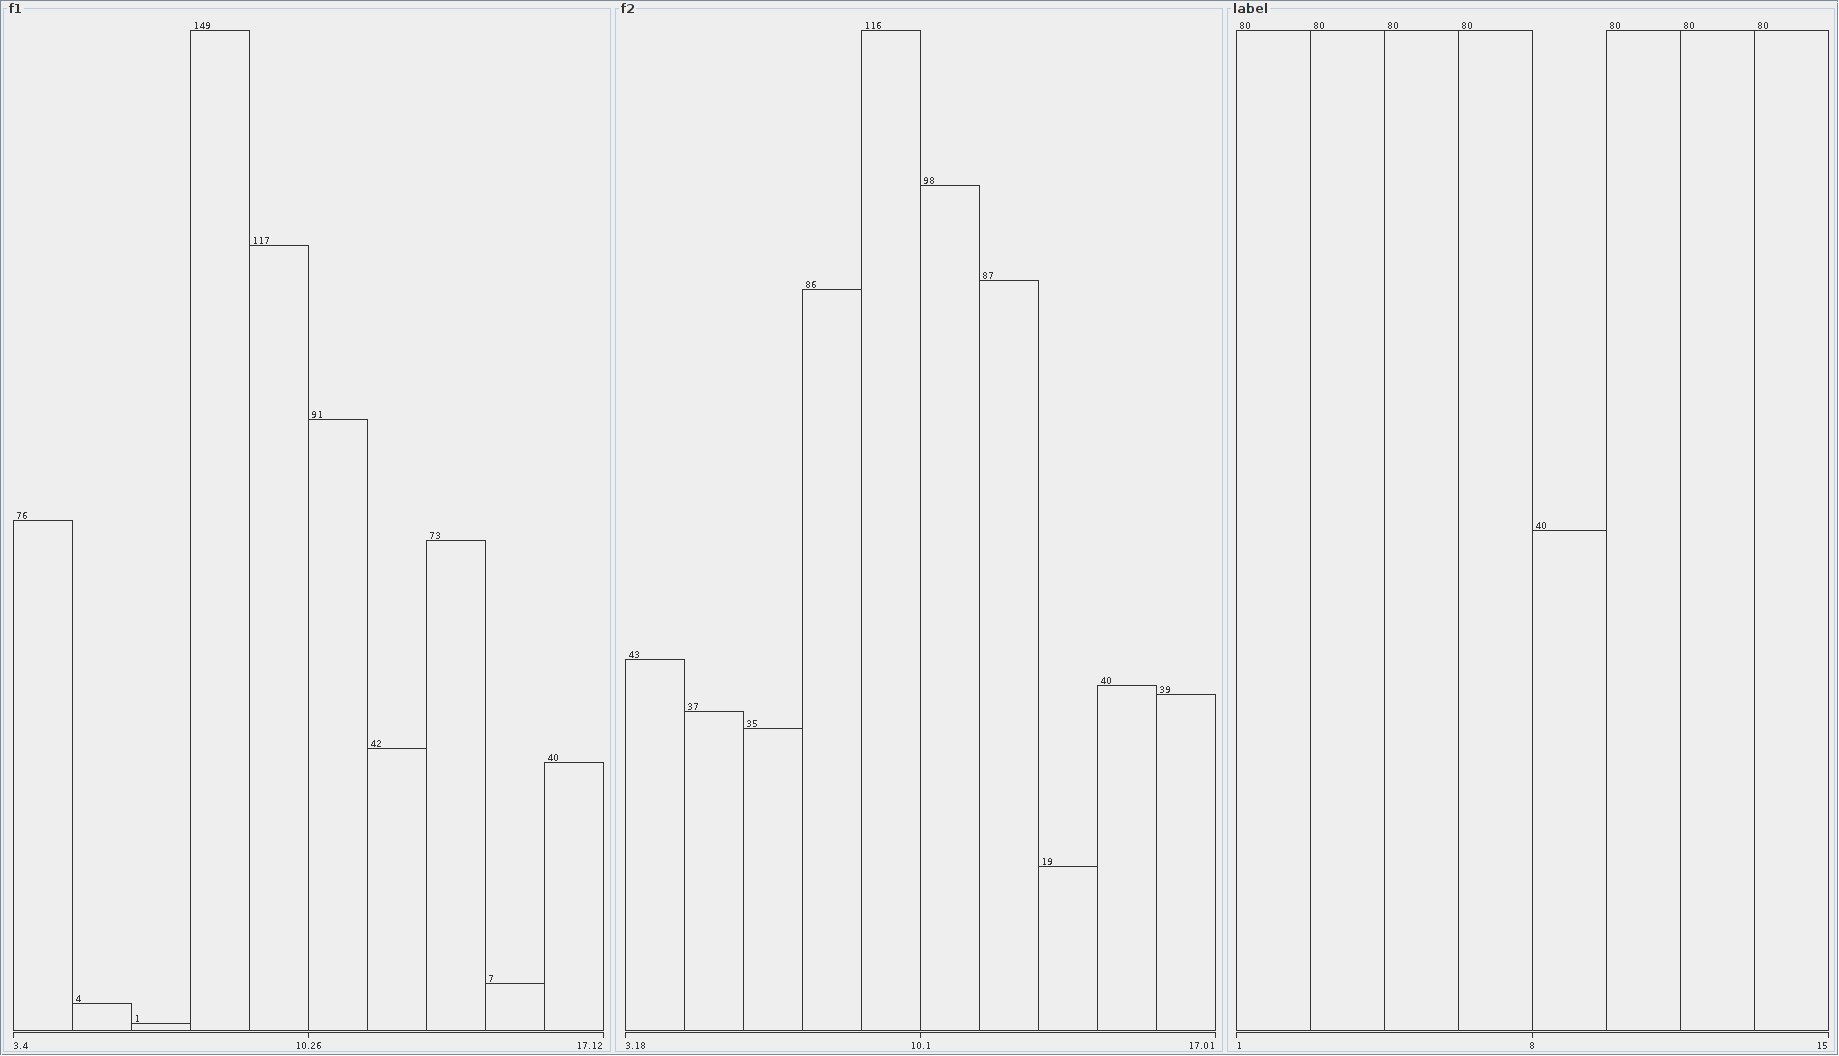
\includegraphics[width=0.8\textwidth]{R15}\label{fig:f1}}
  \hfill
  \subfloat{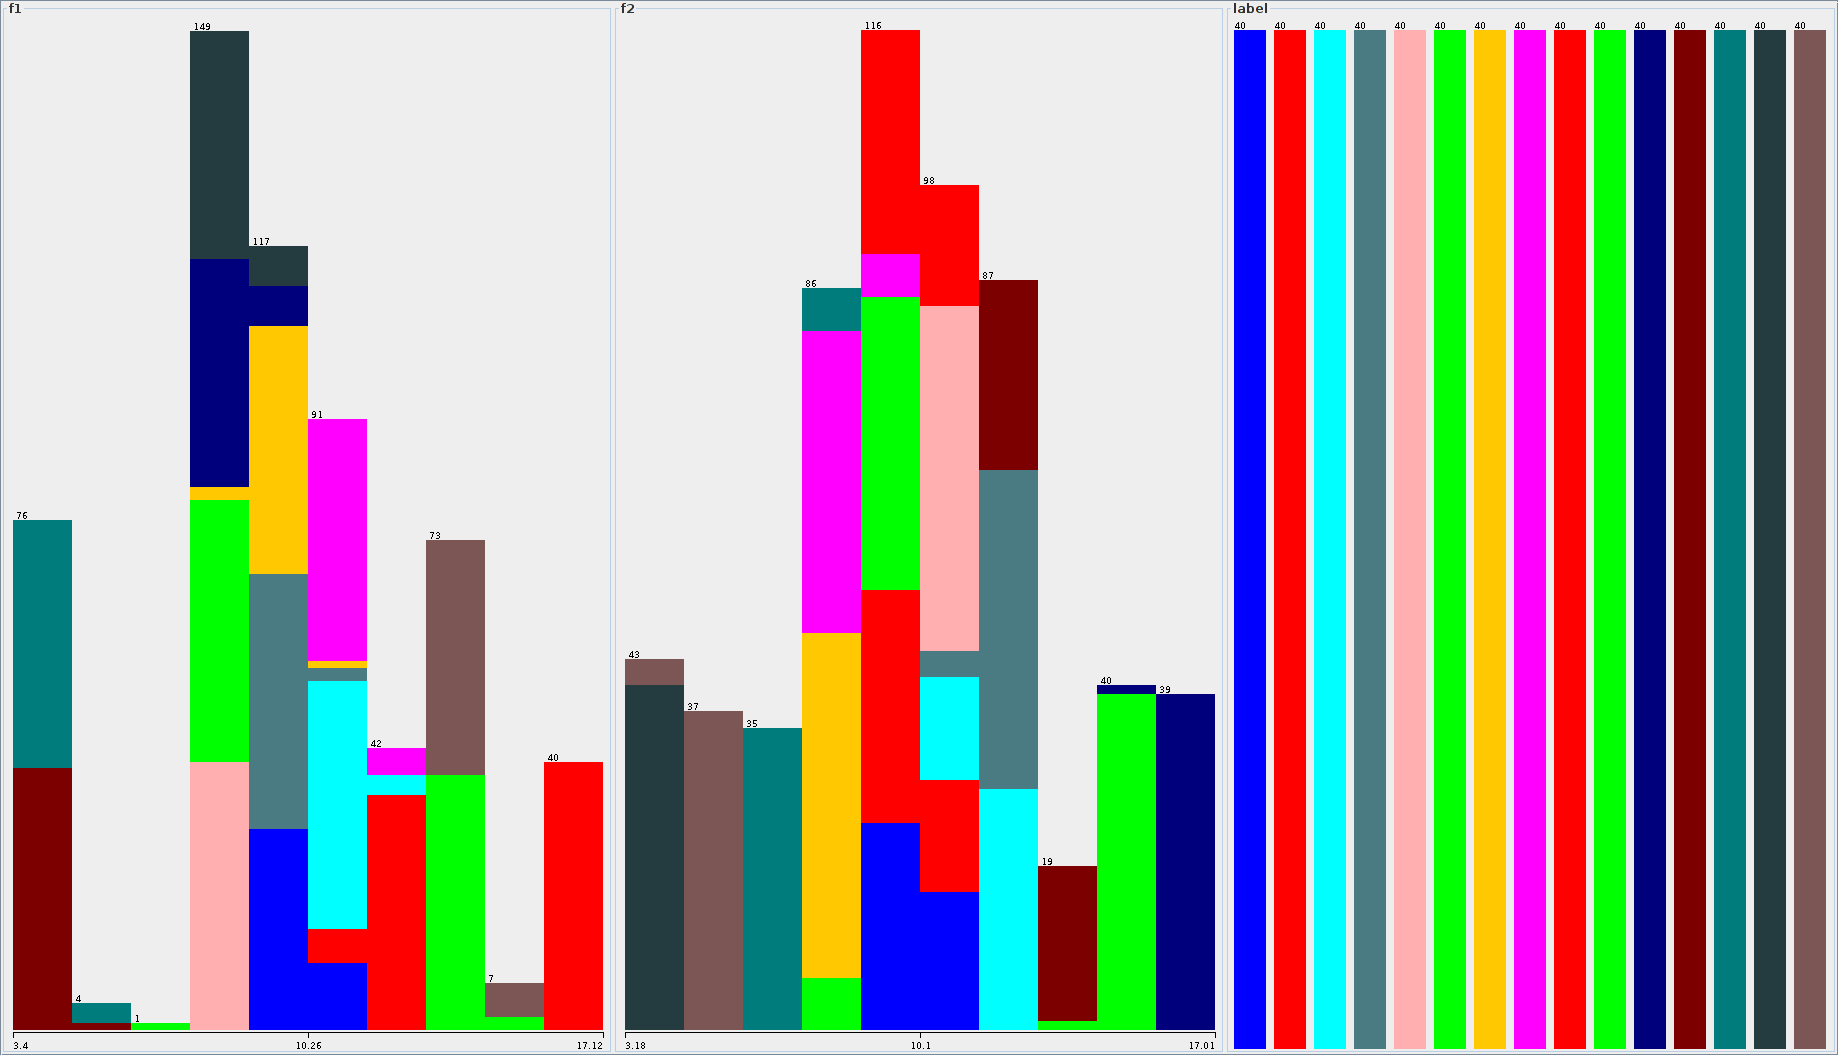
\includegraphics[width=0.8\textwidth]{R15_4}\label{fig:f2}}
  \caption*{Classwise distribution of datapoints along features}
\end{figure}

Since the datapoints are well seperated with sufficient between class variance and small in-class variance, K-means can give us very good clustering results, as it is based on the distance from centroids.

Since the points belonging to the same class are densely clusterd together, DBSCAN can give us very good results by appropriately choosing $\epsilon$ and MinPts.

Since the points belonging to the same class are densely clusterd together(less distance between points), Single link hierarchial clustering can give us good results, as it checks for the distance between the nearest datapoints in two clusters before merging them.

Complete Link might not give us a good solution since it merges the clusters having minimum distance between the farthest datapoint in each cluster. Hence, we might reach a solution where in, set of datapoints belonging to one class gets merged with another.

\begin{figure}[H]
  \centering
  \subfloat{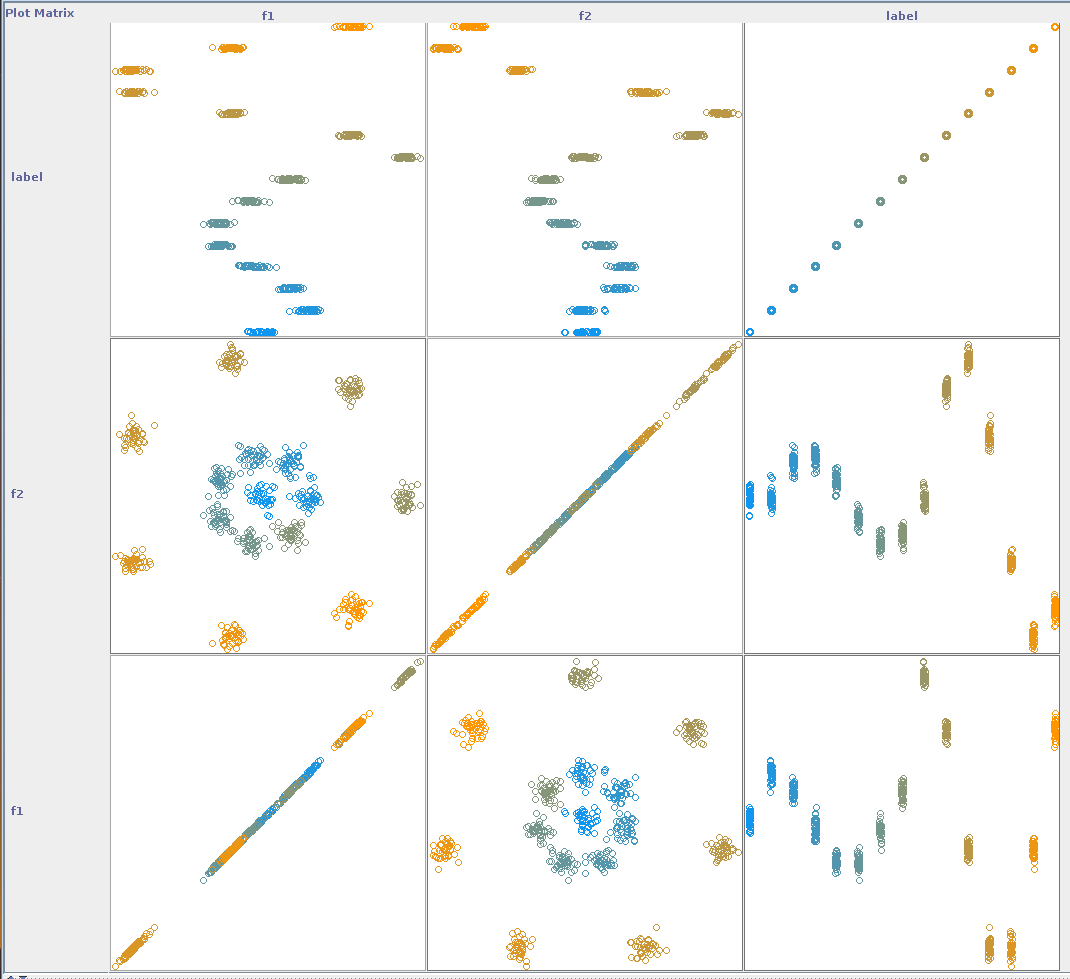
\includegraphics[width=0.7\textwidth]{R15_2}\label{fig:f1}}
  \hfill
  \subfloat{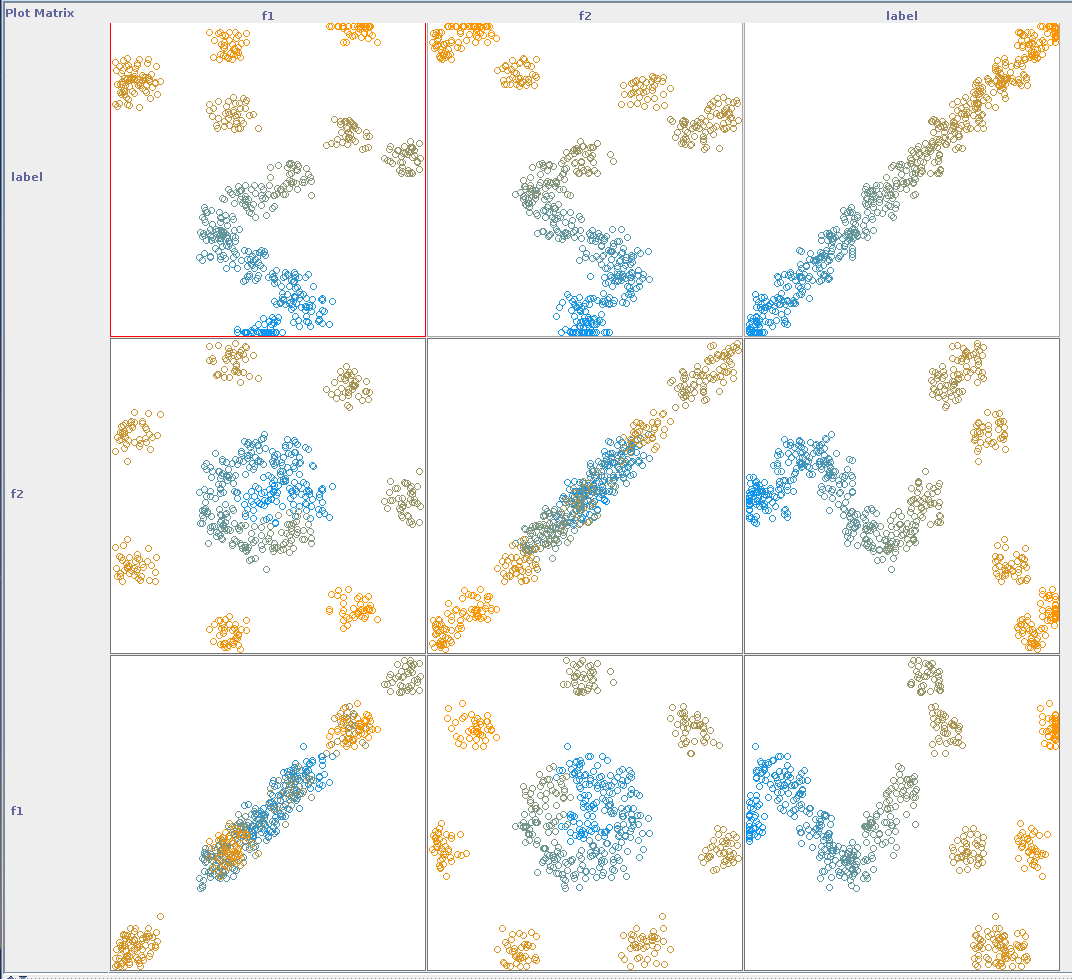
\includegraphics[width=0.7\textwidth]{R15_3}\label{fig:f2}}
  \caption*{Correlation Analysis}
\end{figure}

\subsubsection*{(viii)Spiral}
\begin{figure}[H]
  \centering
  \subfloat{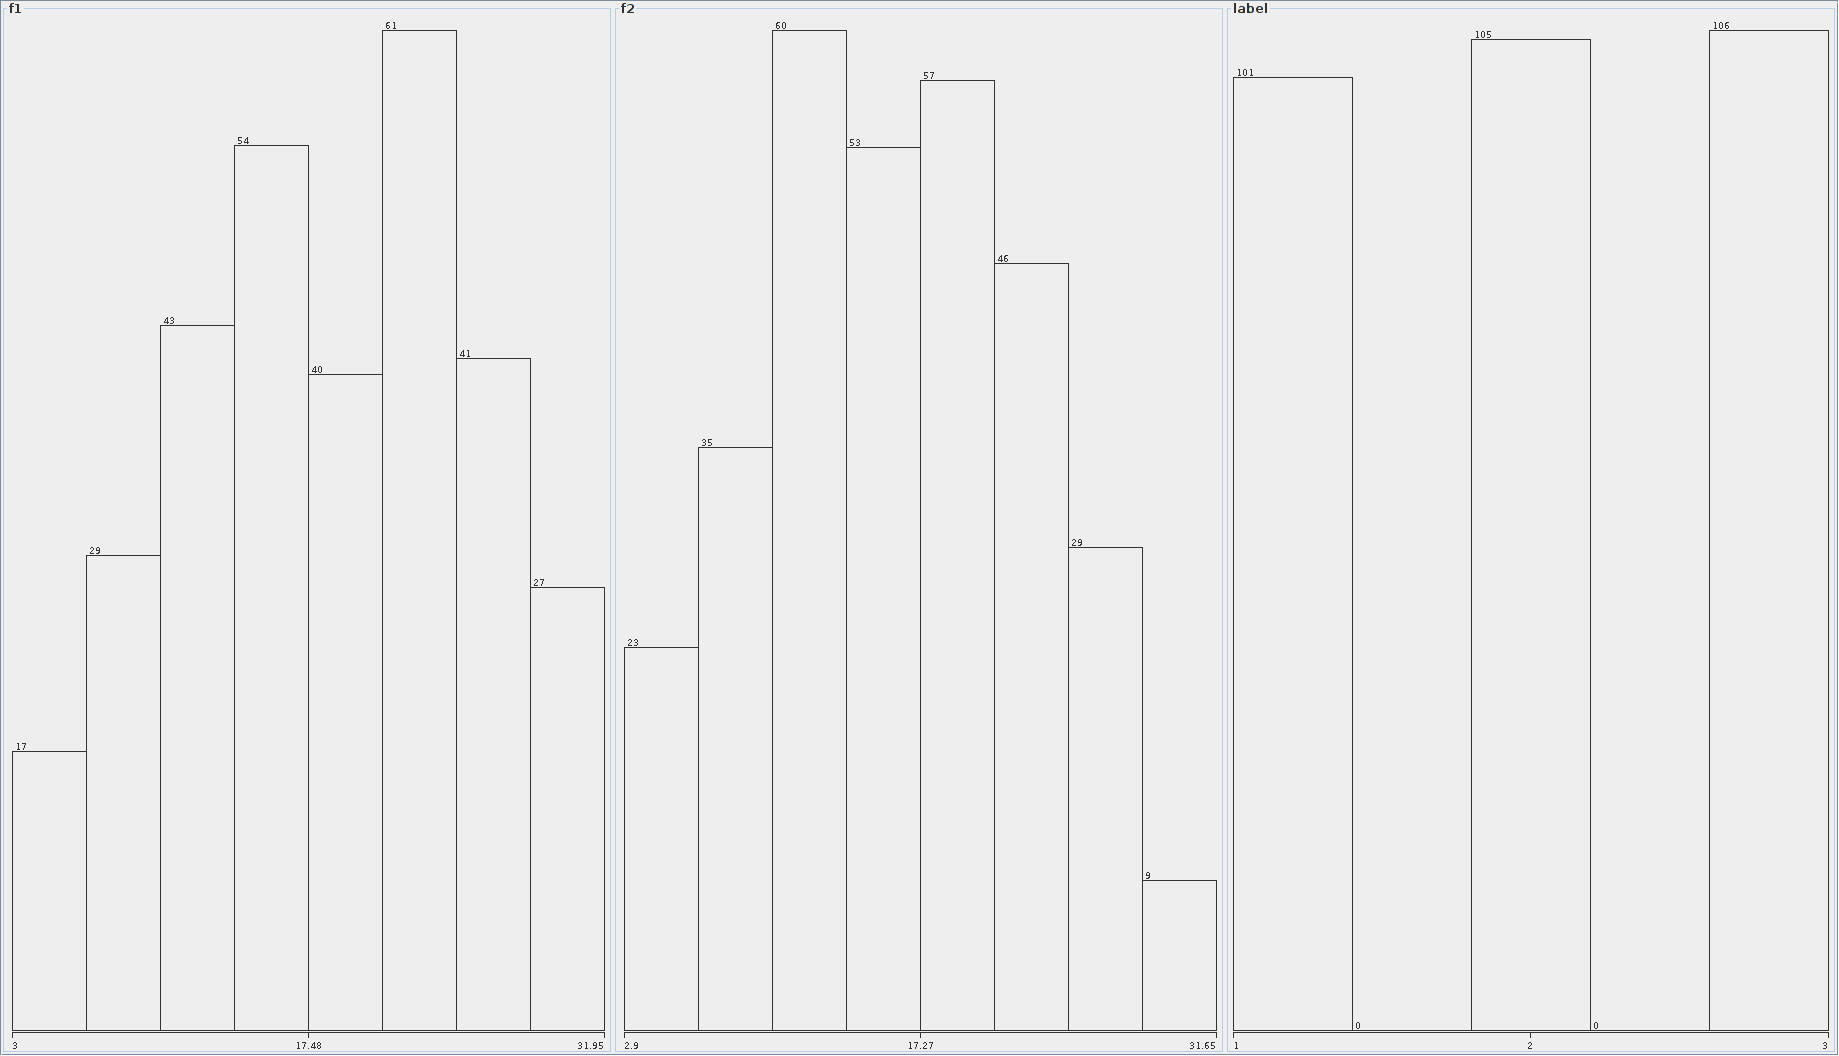
\includegraphics[width=0.8\textwidth]{Spiral}\label{fig:f1}}
  \hfill
  \subfloat{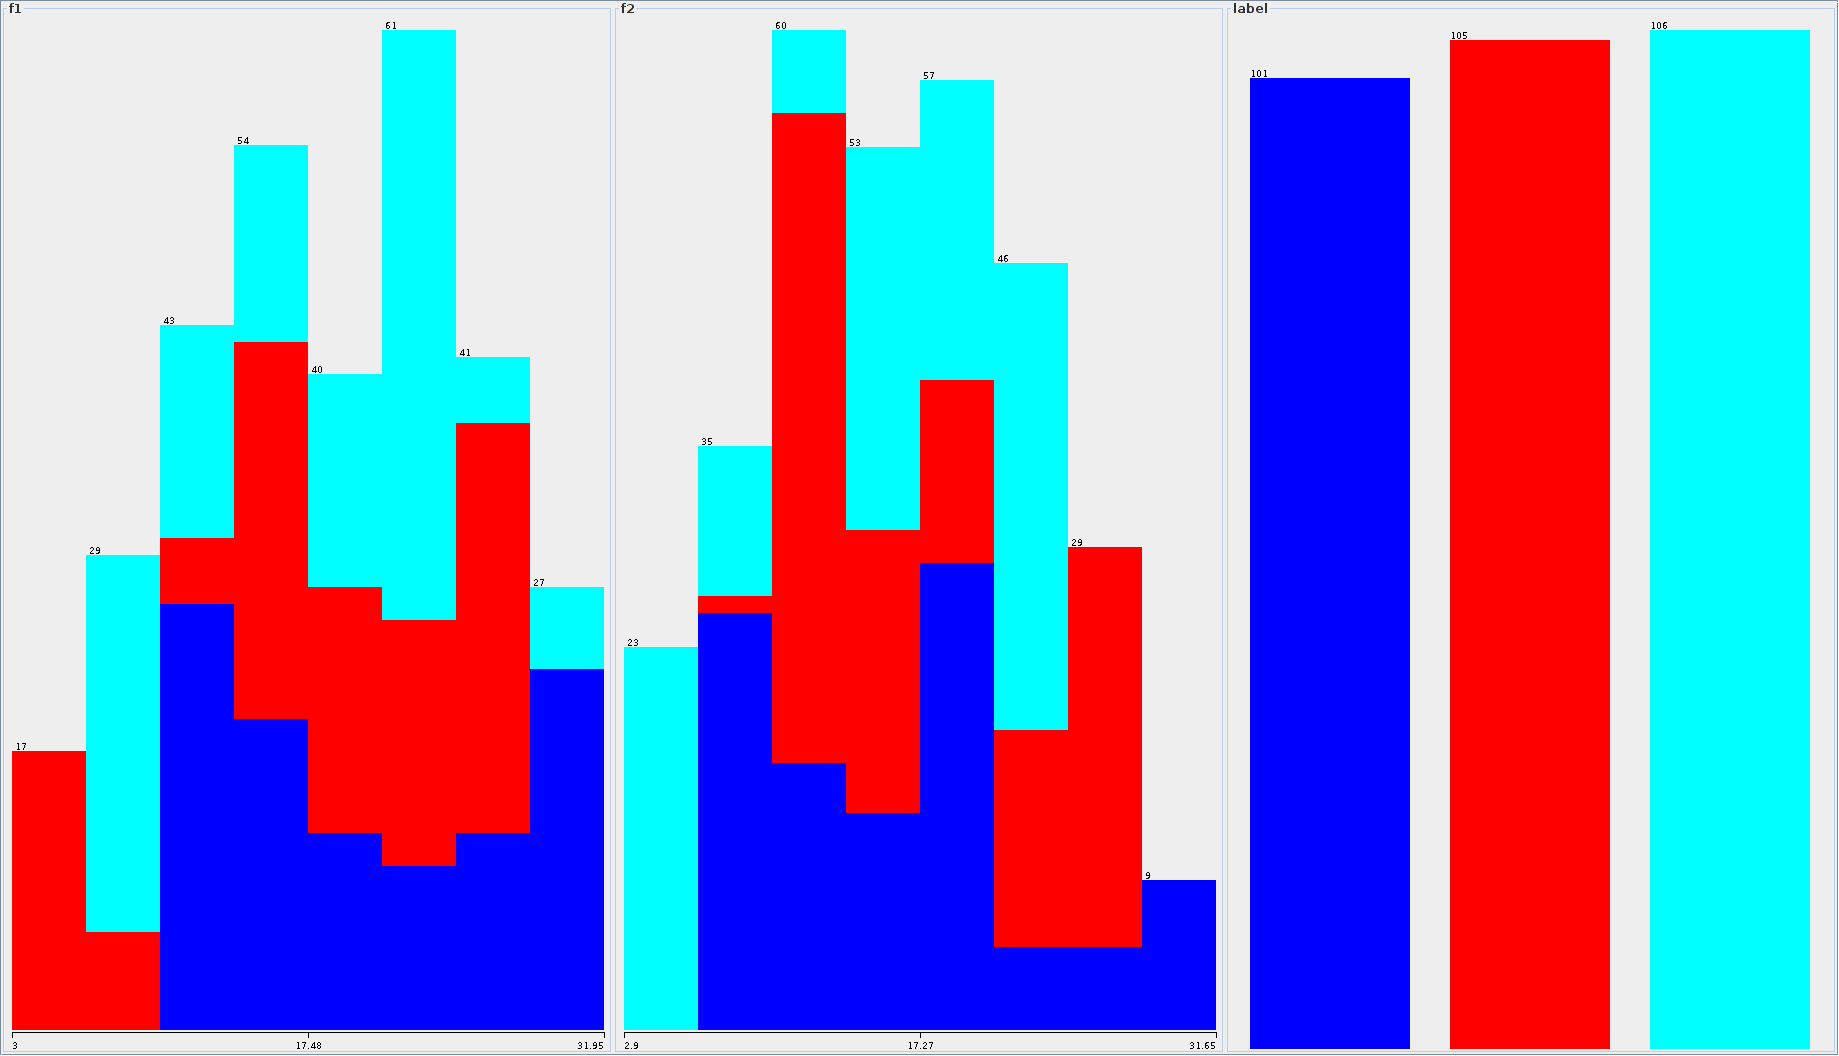
\includegraphics[width=0.8\textwidth]{Spiral4}\label{fig:f2}}
  \caption*{Classwise distribution of datapoints along features}
\end{figure}

K-means would converge to a very bad clustering results as the classes are spiralling one another. Hence K-means cannot be used to identify the classes, as the optimum centroid is in the center of the spiral.

Since the points belonging to the same class are densely clusterd together, DBSCAN can give us very good results by appropriately choosing $\epsilon$ and MinPts. (Small $\epsilon$ and appropriate MinPts)

Since the classes are in the form of spirals, Single link can give us good clusters for classification.Since the points belonging to the same class are densely clusterd together(less distance between points), Single link hierarchial clustering can give us good results, as it checks for the distance between the nearest datapoints in two clusters before merging them.

Complete Link will give us a very bad solution since it merges the clusters having minimum distance between the farthest datapoint in each cluster. Hence, we will reach a solution where in, set of datapoints belonging to one class gets merged with another.

\begin{figure}[H]
  \centering
  \subfloat{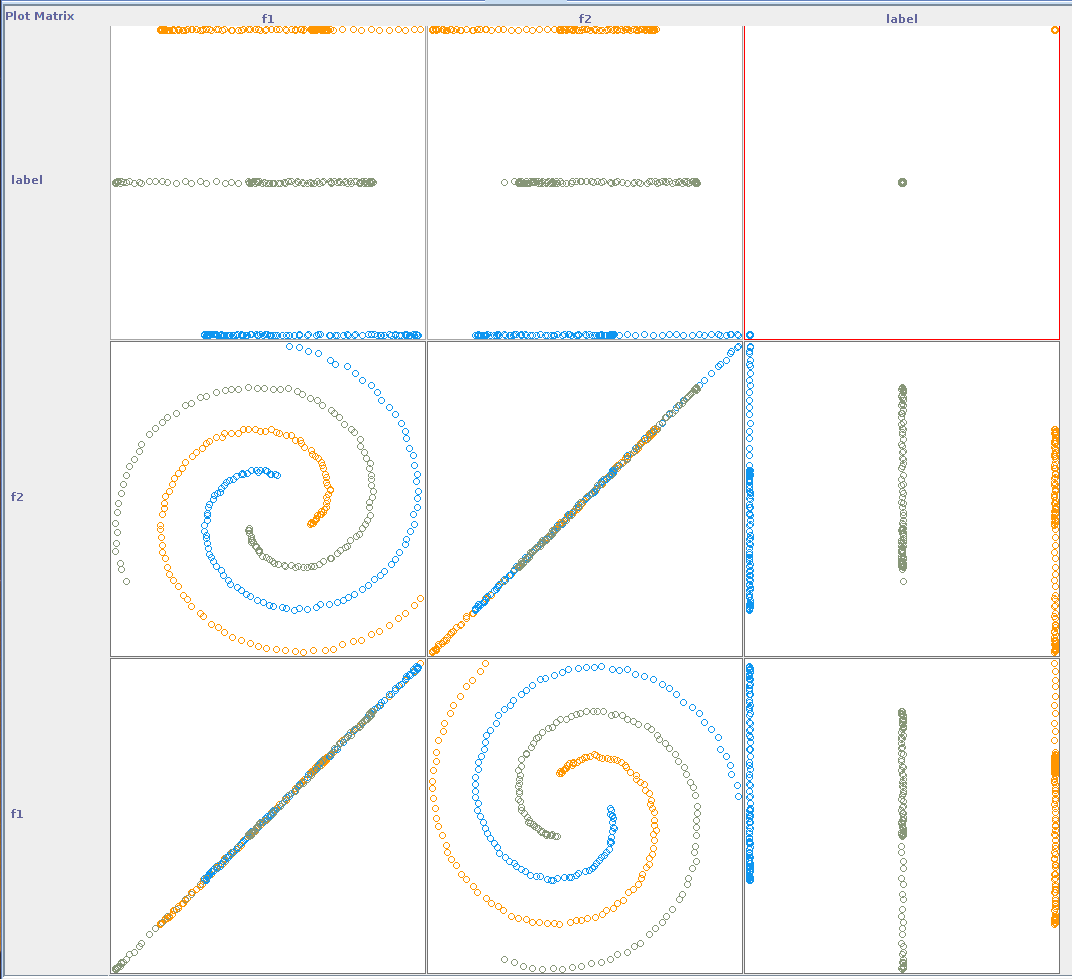
\includegraphics[width=0.7\textwidth]{Spiral2}\label{fig:f1}}
  \hfill
  \subfloat{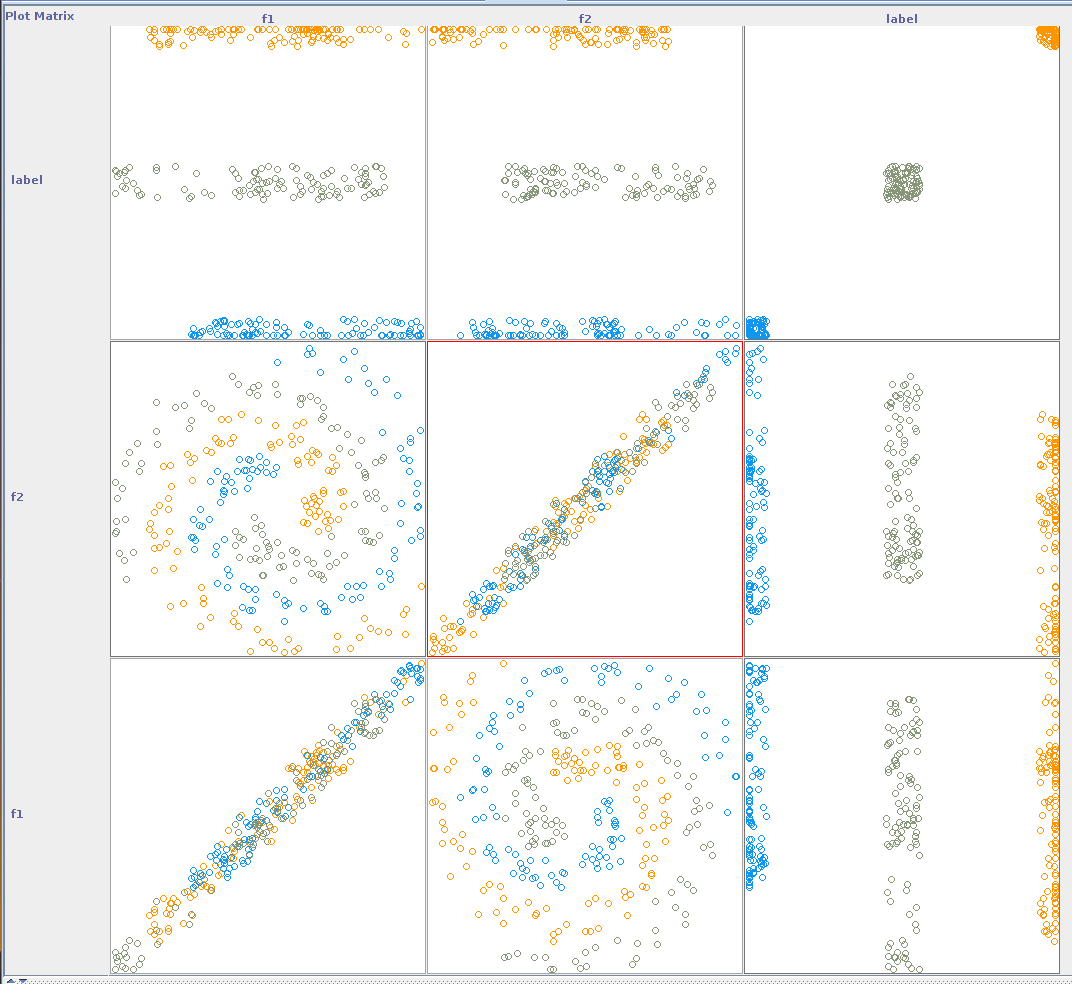
\includegraphics[width=0.6\textwidth]{Spiral3}\label{fig:f2}}
  \caption*{Correlation Analysis}
\end{figure}


\subsection*{3.R15 : K-means and Cluster Purity}
K-means clustering is a type of unsupervised learning, which aims to partition n observations into k clusters in which each observation belongs to the cluster with the nearest mean, serving as a prototype of the cluster.\\

 Purity is a measure of the extent to which clusters contain a single class. It is an evaluation measure for the quality of clustering. It is calculated by counting the number of data points from the most common class in a cluster. and then take the sum over all clusters and divide by the total number of data points. Given some set of clusters M and some set of classes D, both partitioning N data points, purity can be defined as:
 
$$Purity = \frac{1}{N} \sum_{m \epsilon M}\max_{d \epsilon D}|m \cap d|$$

The results of clustering with k=8 is as follows :
\begin{figure}[H]
  \centering
  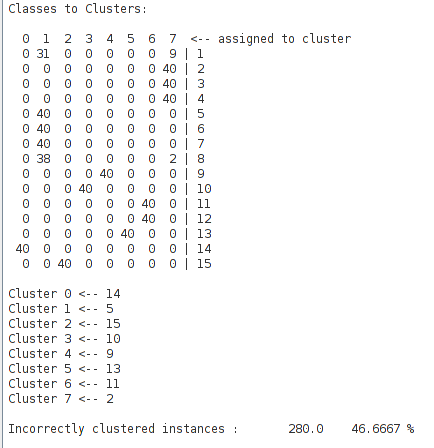
\includegraphics[width=0.8\textwidth]{k-means_8_2}\label{fig:f1}
\end{figure}

\begin{figure}[H]
	\centering
  \includegraphics[width=1\textwidth]{k-means_8}\label{fig:f2}
\end{figure}

The cluster purity for different values of K have been listed below :

\begin{figure}[H]
  \centering
  \subfloat{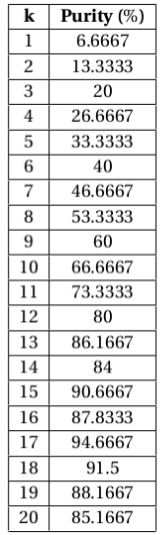
\includegraphics[width=0.2\textwidth]{purity_val}\label{fig:f1}}
  \hfill
  \subfloat{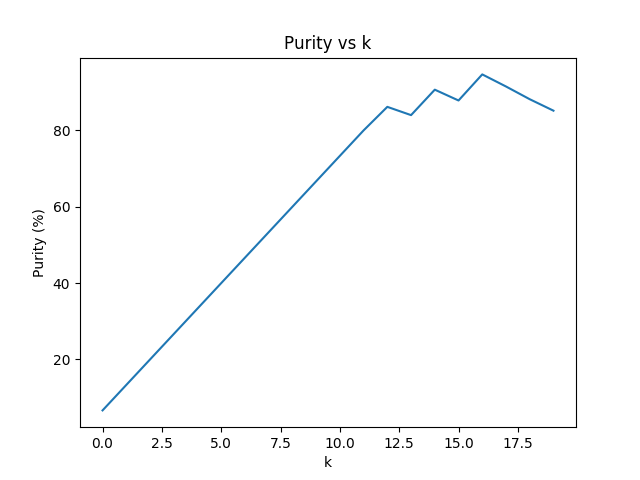
\includegraphics[width=0.75\textwidth]{purity}\label{fig:f2}}
  \caption*{Purity vs No. of Clusters}
\end{figure}

\subsection*{4.Jain : DBSCAN and Cluster Purity}
Density-based spatial clustering of applications with noise (DBSCAN) is a data clustering algorithm which is density based: given a set of points in some space, it groups together points that are closely packed together (points with many nearby neighbors), marking as outliers points that lie alone in low density regions (whose nearest neighbors are too far away).

The variation of Purity with $\epsilon$ and MinPts have been evaluated for some changes of values and the plotted as shown below :
\begin{figure}[H]
\begin{center}
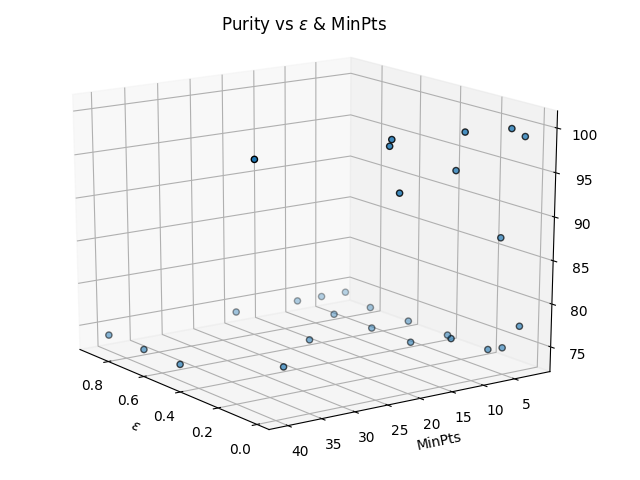
\includegraphics[scale=0.9]{dbscan_1}
\end{center}
\end{figure}

\begin{figure}[H]
	\centering
  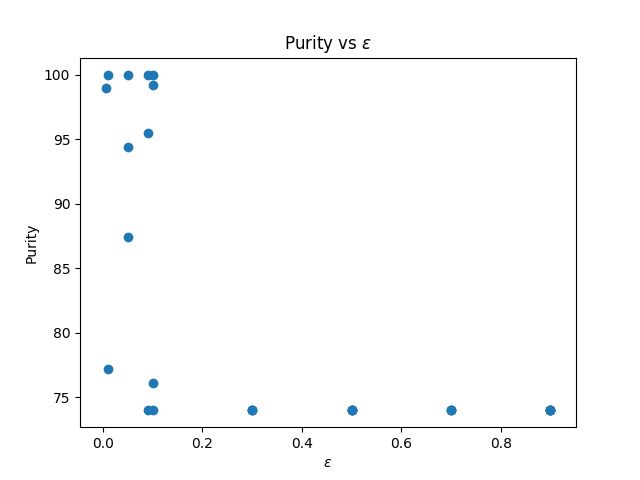
\includegraphics[width=0.7\textwidth]{dbscan_2}\label{fig:f2}
\end{figure}

\begin{figure}[H]
	\centering
  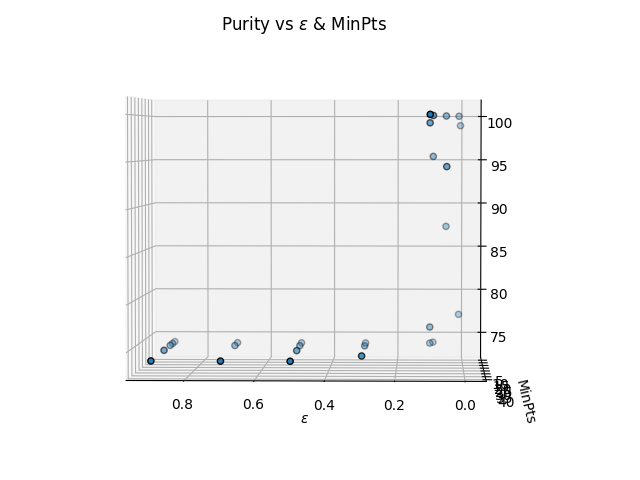
\includegraphics[width=0.9\textwidth]{dbscan_4}\label{fig:f2}
\end{figure}

\begin{figure}[H]
	\centering
  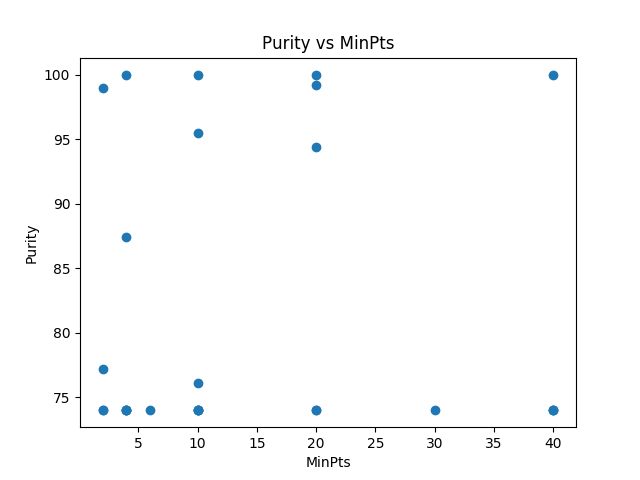
\includegraphics[width=0.7\textwidth]{dbscan_3}\label{fig:f2}
\end{figure}

\begin{figure}[H]
	\centering
  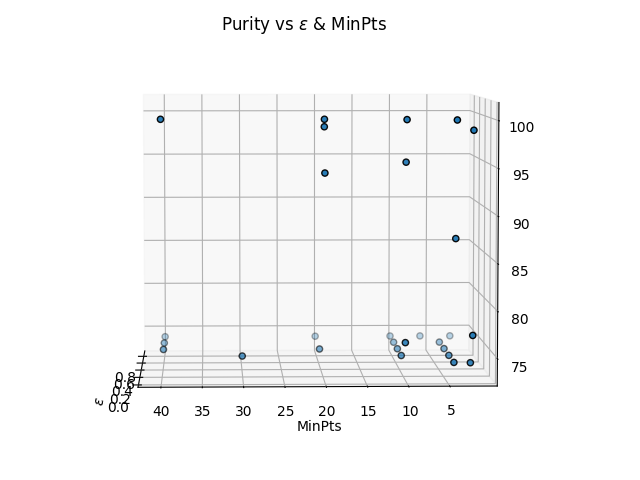
\includegraphics[width=0.9\textwidth]{dbscan_5}\label{fig:f2}
\end{figure}


\subsection*{5. DBSCAN vs Hierarchial CLustering}
Hierarchical clustering is a method of cluster analysis which seeks to build a hierarchy of clusters. The following are the strategies used for hierarchical clustering :
\begin{itemize}
\item Agglomerative: This is a "bottom up" approach: each observation starts in its own cluster, and pairs of clusters are merged as one moves up the hierarchy
\item Divisive: This is a "top down" approach: all observations start in one cluster, and splits are performed recursively as one moves down the hierarchy
\end{itemize}


Usually, the merges and splits are determined in a greedy manner and the results of hierarchical clustering are presented in a dendrogram.


\subsubsection*{(i)Path-based}
\begin{table}[H]
\label{T:equipos}
\begin{center}
\begin{tabular}{| c | c | c | c |}
\hline
\multicolumn{4}{| c |}{\textbf{DBSCAN}}  \\ 
\cline{1-4}
\textbf{$\epsilon$} & \textbf{MinPts} & \textbf{Purity($\%$)} & \textbf{Number of clusters}\\
\hline

0.1  & 4 & 36.6667 & 1 \\ \hline
0.1 & 6 & 37 & 1\\ \hline
0.1 & 10 & 54.3333 & 2\\ \hline
0.1 & 15 & 94.3333 & 2\\ \hline
0.1 & 20 & 98 & 2\\ \hline
0.1 & 25 & 99 & 2\\ \hline
0.1 & 30 & 99.3333 & 2\\ \hline
0.1 & 35 & 99.3333 & 2\\ \hline
0.1 & 40 & 100 & 1\\ \hline

\end{tabular}
\end{center}
\end{table}

But we notice from the output that as we increase the number of MinPts, the number of identified clusters first increases and then reduces and it classifies the low density regions as noise and the number of points classified as noise increases as MinPts increases. Here we haven't been able to find 3 clusters corresponding to the number of class labels due to the choice of the value of $\epsilon$. For $\epsilon = 0.1$, no choice of MinPts give us more than 2 clusters.\\

But say $\epsilon = 0.05$, then we see that for Minpts $=$ 10, we get a purity of 94.3333$\%$ with 3 clusters.\\

\begin{table}[H]
\label{T:equipos}
\begin{center}
\begin{tabular}{| c | c |}
\hline
\multicolumn{2}{| c |}{\textbf{Heirarchial}}  \\ 
\cline{1-2}
\textbf{TYPE} & \textbf{Purity($\%$)} \\
\hline

Single  & 27  \\ \hline
Complete & 70.6667 \\ \hline
Average & 63 \\ \hline
Mean & 70\\ \hline
Centroid & 73.3333 \\ \hline
Ward & 75.3333 \\ \hline
AdjComplete & 64 \\ \hline
NeighborJoining & 36.6667\\ \hline

\end{tabular}
\end{center}
\end{table}

This has been done for Number of Clusters = 3 = Number of Classes\\
From the above observation, WARD gives us the highest purity score for the Path-based dataset.

\subsubsection*{(ii)Spiral}
\begin{table}[H]
\label{T:equipos}
\begin{center}
\begin{tabular}{| c | c | c | c |}
\hline
\multicolumn{4}{| c |}{\textbf{DBSCAN}}  \\ 
\cline{1-4}
\textbf{$\epsilon$} & \textbf{MinPts} & \textbf{Purity($\%$)} & \textbf{Number of clusters}\\
\hline

0.1  & 4 & 100 & 3 \\ \hline
0.1 & 6 & 100 & 3 \\ \hline
0.1 & 10 & 100 & 3 \\ \hline
0.1 & 15 & 100 & 3 \\ \hline
0.1 & 20 & 100 & 3 \\ \hline
0.1 & 25 & 100 & 3 \\ \hline

\end{tabular}
\end{center}
\end{table}

But we notice from the output that as we increase the number of MinPts, it classifies the low density regions as noise and the number of points classified as noise increases as MinPts increases. 

\graphicspath{ {../Dataset/1_Clustering/Visualisations/} }
\begin{figure}[H]
  \centering
  \subfloat[$MinPts = 4$]{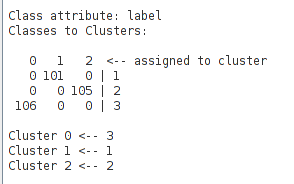
\includegraphics[width=0.5\textwidth]{DB1}}
  \hfill
  \subfloat[$MinPts = 10$]{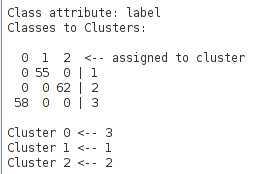
\includegraphics[width=0.5\textwidth]{DB2}}
  \vfill
  \subfloat[$MinPts = 15$]{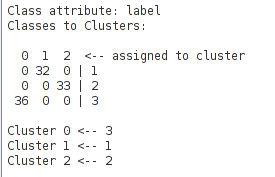
\includegraphics[width=0.5\textwidth]{DB3}}
  \hfill
  \subfloat[$MinPts = 25$]{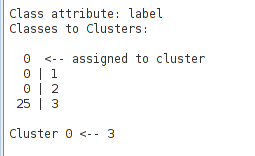
\includegraphics[width=0.5\textwidth]{DB4}}
\end{figure}

Hence for $\epsilon = 0.1$ and  Minpts $=$ 4, we get a purity of 100$\%$ with 3 clusters.\\

\begin{table}[H]
\label{T:equipos}
\begin{center}
\begin{tabular}{| c | c |}
\hline
\multicolumn{2}{| c |}{\textbf{Heirarchial}}  \\ 
\cline{1-2}
\textbf{TYPE} & \textbf{Purity($\%$)} \\
\hline

Single  & 100  \\ \hline
Complete & 38.141 \\ \hline
Average & 36.2179 \\ \hline
Mean & 39.1026\\ \hline
Centroid & 40.3846 \\ \hline
Ward & 40.0641 \\ \hline
AdjComplete & 35.5769 \\ \hline
NeighborJoining & 33.9744\\ \hline

\end{tabular}
\end{center}
\end{table}

This has been done for Number of Clusters = 3 = Number of Classes. \\
From the above observation, SINGLE gives us the highest purity score for the Spiral dataset.

\subsubsection*{(iii)Flames}
\begin{table}[H]
\label{T:equipos}
\begin{center}
\begin{tabular}{| c | c | c | c |}
\hline
\multicolumn{4}{| c |}{\textbf{DBSCAN}}  \\ 
\cline{1-4}
\textbf{$\epsilon$} & \textbf{MinPts} & \textbf{Purity($\%$)} & \textbf{Number of clusters}\\
\hline

0.1  & 4 & 62.5833 & 1 \\ \hline
0.1 & 6 & 64.5833 & 1 \\ \hline
0.1 & 10 & 99.1667 & 2 \\ \hline
0.1 & 15 & 91.25 & 3 \\ \hline
0.1 & 20 & 100 & 1 \\ \hline

\end{tabular}
\end{center}
\end{table}

But we notice from the output that as we increase the number of MinPts, it classifies the low density regions as noise and the number of points classified as noise increases as MinPts increases. 

\graphicspath{ {../Dataset/1_Clustering/Visualisations/} }
\begin{figure}[H]
  \centering
  \subfloat[$MinPts = 15$]{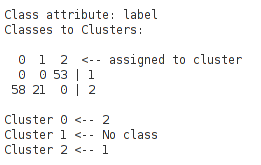
\includegraphics[width=0.5\textwidth]{DB5}}
  \hfill
  \subfloat[$MinPts = 20$]{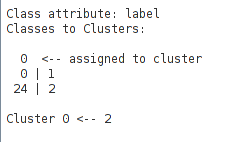
\includegraphics[width=0.5\textwidth]{DB6}}
\end{figure}

\graphicspath{ {../Dataset/1_Clustering/Visualisations/} }
\begin{figure}[H]
  \centering
  \subfloat[$MinPts = 6$]{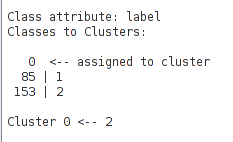
\includegraphics[width=0.5\textwidth]{DB7}}
  \hfill
  \subfloat[$MinPts = 10$]{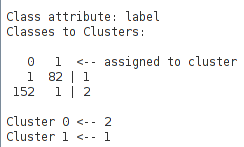
\includegraphics[width=0.5\textwidth]{DB8}}
\end{figure}

Hence for $\epsilon = 0.1$ and  Minpts $=$ 10, we get a purity of 99.1667$\%$ with 2 clusters.\\

\begin{table}[H]
\label{T:equipos}
\begin{center}
\begin{tabular}{| c | c |}
\hline
\multicolumn{2}{| c |}{\textbf{Heirarchial}}  \\ 
\cline{1-2}
\textbf{TYPE} & \textbf{Purity($\%$)} \\
\hline

Single  & 64.5883 \\ \hline
Complete & 51.6667 \\ \hline
Average & 83.3333 \\ \hline
Mean & 92.0833\\ \hline
Centroid & 64.5833 \\ \hline
Ward & 100 \\ \hline
AdjComplete & 64.1667 \\ \hline
NeighborJoining & 63.75\\ \hline

\end{tabular}
\end{center}
\end{table}

This has been done for Number of Clusters = 2 = Number of Classes. \\
From the above observation, WARD gives us the highest purity score for the Flames dataset.

\subsubsection*{Inference}
\begin{table}[H]
\label{T:equipos}
\begin{center}
\begin{tabular}{| c | c | c |}
\hline
\textbf{Class} & \textbf{Clustering Algorithm} & \textbf{Reason} \\
\hline

Path-based  & DBSCAN ($\epsilon =0.05 \& MinPts = 10)$) & We get better purity value with 3 clusters \\ \hline
Spiral & DBSCAN $\&$ Hierarchial SINGLE & We get 100$\%$ purity value using both \\ \hline
Flames & Hierarchial SINGLE & We get 100$\%$ purity value with 2 clusters \\ \hline

\end{tabular}
\end{center}
\end{table}

\subsection*{6. D31 Dataset}
\subsubsection*{K-Means}
On using sklearn kmeans package, the following results were obtained :
\begin{table}[H]
\label{T:equipos}
\begin{center}
\begin{tabular}{| c | c |}
\hline
\textbf{k} & \textbf{Rand Index} \\
\hline

31 & 0.952873445973 \\ \hline
32 & 0.945115106759 \\ \hline
40 & 0.858723966641 \\ \hline
50 & 0.774456828936 \\ \hline
70 & 0.604866171665 \\ \hline

\end{tabular}
\end{center}
\end{table}

On using Weka :o
The data has 31 classes and 3100 datapoints. On directly running K-means with k=32 and supplying the class labels for comparison, convergence wasn't obtained even after leaving the code running for more than a day on Weka, even if we specify the number of iterations as 1 (which is the lowest). k=32 :

\begin{figure}[H]
	\centering
  \includegraphics[width=1\textwidth]{6a}{\label{k=32: f1 vs f2}}
\end{figure}

\begin{figure}[H]
	\centering
  \includegraphics[width=1\textwidth]{6b}{\label{k=32: cluster vs label}}
\end{figure}

Hence, just the clustering has been implemented and the outcome of k=32 has been shown. On clicking on the clustered points, we get to know the cluster they belong to and for k<31 we see that there are datapoints close to one another that have been classified in different clusters. There are points farther away that has been classified as belonging to the same cluster as well. Hence for k=32, we'll mostly not be able to capture a good fraction of data belonging to different classes, but the amount of miss-classifications would reduce by clustering using a larger value of k because, as k increases, points that are more densly close to one another would be classified as belonging to the same cluster and the the points that are relatively farther would be classified in different clusters. Hence, by merging the appropriate clusters, we can get almost all the 31 real clusters by choosing an appropriate k value.\\



We also see from the cluster vs label figure that the points have been clustered randomly and not necessarily linearly.\\\\
For k=50 :

\begin{figure}[H]
	\centering
  \includegraphics[width=0.9\textwidth]{6c}{\label{k=50: f1 vs f2}}
\end{figure}

\begin{figure}[H]
	\centering
  \includegraphics[width=0.9\textwidth]{6d}{\label{k=50: cluster vs label}}
\end{figure}

For k=10 :
\begin{figure}[H]
	\centering
  \includegraphics[width=0.9\textwidth]{k_10}{\label{k=50: cluster vs label}}
\end{figure}


\subsubsection*{DBSCAN}
Even DBSCAN wasn't converging for small values of $\epsilon$ and larger values of MinPts. DBSCAN is found to perform poorly in most of the cases where clustering was possible. Example is as follows :\\\\
For $\epsilon = 0.05$ and MinPts = 45(maximum possible for the given $\epsilon$) :
\begin{figure}[H]
	\centering
  \includegraphics[width=0.8\textwidth]{6db}
\end{figure}

\begin{figure}[H]
	\centering
  \includegraphics[width=1\textwidth]{6db2}{\label{k=50: f1 vs f2}}
\end{figure}

DBSCAN worked very well for $\epsilon = 0.03$ and MinPts = 45 as shown below :
\begin{figure}[H]
	\centering
  \includegraphics[width=1\textwidth]{6db3}
\end{figure}

\begin{figure}[H]
	\centering
  \includegraphics[width=1\textwidth]{6db4}
\end{figure}
But actually, it considered several points as Noise points and hence we get a very good putiry score. \\

But $\epsilon = 0.03$ and MinPts < 45, it didn't converge even after running for a long time.

\subsubsection*{Hierarchial Clustering : WARD linkage}
The results are as follows :\\
Number of Clusters = 10 :
\begin{figure}[H]
	\centering
  \includegraphics[width=1\textwidth]{6db6}
\end{figure}

Number of Clusters = 20 :
\begin{figure}[H]
	\centering
  \includegraphics[width=1.2\textwidth]{6db7}
\end{figure}


\newpage
\section*{Naive Bayes}
Design and implementation of a Bayesian Spam Filter that classifies email messages as either spam(unwanted) or ham (useful), that is, $y_{i} \epsilon$ ${spam, ham}$ using a Naive Bayes Classifier for the following four scenarios:

\subsection*{1. Maximum Likelihood Estimation assuming likelihood: Multinomial}
This has been implemented using sklearn as well as from scratch in python.
\subsubsection*{From Scratch}
The results obtained are as follows :
\begin{table}[H]
\label{T:equipos}
\begin{center}
\begin{tabular}{| c | c | c | c |}
\hline
\textbf{Labels} & \multicolumn{3}{ c |}{\textbf{Per Class Estimates}}  \\ 
\cline{2-4}
& \textbf{Precision} & \textbf{Recall} & \textbf{F-measure} \\
\hline

Legit & 98 & 95 & 97  \\ \hline
Spam 2 & 94 & 98 & 96 \\ \hline
Avg & 96 & 96 & 96 \\ \hline

\end{tabular}
\end{center}
\end{table}

The PR curve has been plotted by giving the difference of the calculated scores with the minimum of all scores and dividing by modulus of the minimum.

PR Curve for spam :
\graphicspath{ {../Dataset/2_NaiveBayes/Visualisations/} }
\begin{figure}[H]
	\centering
  \includegraphics[width=0.9\textwidth]{mul}
\end{figure}

On calculating the probability as the score of legit divided by the score of legit and spam (since score is negative, we take the class with the less negative score and hence the relation), the result obtained is as follows :
\begin{table}[H]
\label{T:equipos}
\begin{center}
\begin{tabular}{| c | c | c | c |}
\hline
\textbf{Labels} & \multicolumn{3}{ c |}{\textbf{Per Class Estimates}}  \\ 
\cline{2-4}
& \textbf{Precision} & \textbf{Recall} & \textbf{F-measure} \\
\hline

Legit & 97 & 97 & 97  \\ \hline
Spam 2 & 96 & 96 & 96 \\ \hline
Avg & 96 & 96 & 96 \\ \hline

\end{tabular}
\end{center}
\end{table}

PR Curve for spam :
\graphicspath{ {../Dataset/2_NaiveBayes/Visualisations/} }
\begin{figure}[H]
	\centering
  \includegraphics[width=0.9\textwidth]{mult}
\end{figure}

\subsubsection*{Using sklearn}
The results obtained are as follows :
\begin{table}[H]
\label{T:equipos}
\begin{center}
\begin{tabular}{| c | c | c | c |}
\hline
\textbf{Labels} & \multicolumn{3}{ c |}{\textbf{Per Class Estimates}}  \\ 
\cline{2-4}
& \textbf{Precision} & \textbf{Recall} & \textbf{F-measure} \\
\hline

Spam & 94 & 95 & 94  \\ \hline
Legit 2 & 94 & 92 & 93 \\ \hline
Avg & 94 & 94 & 94 \\ \hline

\end{tabular}
\end{center}
\end{table}

PR Curve for spam :
\graphicspath{ {../Dataset/2_NaiveBayes/Visualisations/} }
\begin{figure}[H]
	\centering
  \includegraphics[width=0.9\textwidth]{1}
\end{figure}

\subsection*{2. Maximum Likelihood Estimation assuming likelihood: Bernoulli}

The results obtained are as follows :
\begin{table}[H]
\label{T:equipos}
\begin{center}
\begin{tabular}{| c | c | c | c |}
\hline
\textbf{Labels} & \multicolumn{3}{ c |}{\textbf{Per Class Estimates}}  \\ 
\cline{2-4}
& \textbf{Precision} & \textbf{Recall} & \textbf{F-measure} \\
\hline

Legit & 91 & 98 & 94  \\ \hline
Spam 2 & 98 & 88 & 92 \\ \hline
Avg & 94 & 94 & 94 \\ \hline

\end{tabular}
\end{center}
\end{table}

PR Curve for spam :
\graphicspath{ {../Dataset/2_NaiveBayes/Visualisations/} }
\begin{figure}[H]
	\centering
  \includegraphics[width=0.9\textwidth]{2}
\end{figure}

\subsection*{3. Bayesian Parameter Estimation assuming the prior: Dirichlet}

The Dirichlet distribution is given by,
\graphicspath{ {../Dataset/2_NaiveBayes/Visualisations/} }
\begin{figure}[H]
	\centering
  \includegraphics[width=0.55\textwidth]{dirichlet}
\end{figure}

The conditioning on each word is given by,
\graphicspath{ {../Dataset/2_NaiveBayes/Visualisations/} }
\begin{figure}[H]
	\centering
  \includegraphics[width=0.55\textwidth]{dirch}
\end{figure}

when the number of words in the vocabulary is K. Here, I have defined twi different Dirichlet distribution for the two classes (Spam and Legit) and hence estimated the the class of each document. The code  has been written from scratch and is a variation of the Multinomial Naive Bayes algorithm.

The PR curve has been plotted by giving the difference of the calculated scores with the minimum of all scores and dividing by modulus of the minimum.

The results obtained are as follows :\\
First run :
\begin{table}[H]
\label{T:equipos}
\begin{center}
\begin{tabular}{| c | c | c | c |}
\hline
\textbf{Labels} & \multicolumn{3}{ c |}{\textbf{Per Class Estimates}}  \\ 
\cline{2-4}
& \textbf{Precision} & \textbf{Recall} & \textbf{F-measure} \\
\hline

Spam & 95 & 94 & 94  \\ \hline
Legit & 94 & 92 & 93 \\ \hline
Avg & 94 & 94 & 94 \\ \hline

\end{tabular}
\end{center}
\end{table}

PR Curve for spam :
\graphicspath{ {../Dataset/2_NaiveBayes/Visualisations/} }
\begin{figure}[H]
	\centering
  	\includegraphics[width=0.9\textwidth]{dr11}
\end{figure}


Second run :
\begin{table}[H]
\label{T:equipos}
\begin{center}
\begin{tabular}{| c | c | c | c |}
\hline
\textbf{Labels} & \multicolumn{3}{ c |}{\textbf{Per Class Estimates}}  \\ 
\cline{2-4}
& \textbf{Precision} & \textbf{Recall} & \textbf{F-measure} \\
\hline

Spam & 97 & 97 & 97  \\ \hline
Legit & 96 & 96 & 96 \\ \hline
Avg & 96 & 96 & 96 \\ \hline

\end{tabular}
\end{center}
\end{table}

PR Curve for spam :
\graphicspath{ {../Dataset/2_NaiveBayes/Visualisations/} }
\begin{figure}[H]
	\centering
  \includegraphics[width=0.9\textwidth]{dr2}
\end{figure}

Third run :
\begin{table}[H]
\label{T:equipos}
\begin{center}
\begin{tabular}{| c | c | c | c |}
\hline
\textbf{Labels} & \multicolumn{3}{ c |}{\textbf{Per Class Estimates}}  \\ 
\cline{2-4}
& \textbf{Precision} & \textbf{Recall} & \textbf{F-measure} \\
\hline

Spam & 92 & 97 & 94  \\ \hline
Legit & 96 & 90 & 92 \\ \hline
Avg & 94 & 94 & 94 \\ \hline

\end{tabular}
\end{center}
\end{table}

PR Curve for spam :
\graphicspath{ {../Dataset/2_NaiveBayes/Visualisations/} }
\begin{figure}[H]
	\centering
  \includegraphics[width=0.9\textwidth]{dr3}
\end{figure}

Fourth run :
\begin{table}[H]
\label{T:equipos}
\begin{center}
\begin{tabular}{| c | c | c | c |}
\hline
\textbf{Labels} & \multicolumn{3}{ c |}{\textbf{Per Class Estimates}}  \\ 
\cline{2-4}
& \textbf{Precision} & \textbf{Recall} & \textbf{F-measure} \\
\hline

Spam & 94 & 97 & 95  \\ \hline
Legit & 96 & 92 & 94 \\ \hline
Avg & 95 & 95 & 95 \\ \hline

\end{tabular}
\end{center}
\end{table}

PR Curve for spam :
\graphicspath{ {../Dataset/2_NaiveBayes/Visualisations/} }
\begin{figure}[H]
	\centering
  \includegraphics[width=0.9\textwidth]{dr4}
\end{figure}

Fifth run :
\begin{table}[H]
\label{T:equipos}
\begin{center}
\begin{tabular}{| c | c | c | c |}
\hline
\textbf{Labels} & \multicolumn{3}{ c |}{\textbf{Per Class Estimates}}  \\ 
\cline{2-4}
& \textbf{Precision} & \textbf{Recall} & \textbf{F-measure} \\
\hline

Legit & 95 & 95 & 95  \\ \hline
Spam & 94 & 94 & 94 \\ \hline
Avg & 95 & 95 & 95 \\ \hline

\end{tabular}
\end{center}
\end{table}

PR Curve for spam :
\graphicspath{ {../Dataset/2_NaiveBayes/Visualisations/} }
\begin{figure}[H]
	\centering
  \includegraphics[width=0.9\textwidth]{dr5}
\end{figure}


Sixth run :
\begin{table}[H]
\label{T:equipos}
\begin{center}
\begin{tabular}{| c | c | c | c |}
\hline
\textbf{Labels} & \multicolumn{3}{ c |}{\textbf{Per Class Estimates}}  \\ 
\cline{2-4}
& \textbf{Precision} & \textbf{Recall} & \textbf{F-measure} \\
\hline

Legit & 98 & 97 & 98  \\ \hline
Spam & 96 & 98 & 97 \\ \hline
Avg & 97 & 97 & 97 \\ \hline

\end{tabular}
\end{center}
\end{table}

PR Curve for spam :
\graphicspath{ {../Dataset/2_NaiveBayes/Visualisations/} }
\begin{figure}[H]
	\centering
  \includegraphics[width=0.9\textwidth]{dr6}
\end{figure}

Seventh run :
\begin{table}[H]
\label{T:equipos}
\begin{center}
\begin{tabular}{| c | c | c | c |}
\hline
\textbf{Labels} & \multicolumn{3}{ c |}{\textbf{Per Class Estimates}}  \\ 
\cline{2-4}
& \textbf{Precision} & \textbf{Recall} & \textbf{F-measure} \\
\hline

Spam & 98 & 95 & 97  \\ \hline
Legit & 94 & 98 & 96 \\ \hline
Avg & 96 & 96 & 96 \\ \hline

\end{tabular}
\end{center}
\end{table}

PR Curve for spam :
\graphicspath{ {../Dataset/2_NaiveBayes/Visualisations/} }
\begin{figure}[H]
	\centering
  \includegraphics[width=0.9\textwidth]{dr7}
\end{figure}

Eighth run :
\begin{table}[H]
\label{T:equipos}
\begin{center}
\begin{tabular}{| c | c | c | c |}
\hline
\textbf{Labels} & \multicolumn{3}{ c |}{\textbf{Per Class Estimates}}  \\ 
\cline{2-4}
& \textbf{Precision} & \textbf{Recall} & \textbf{F-measure} \\
\hline

Legit & 94 & 98 & 96  \\ \hline
Spam & 98 & 92 & 95 \\ \hline
Avg & 96 & 95 & 95 \\ \hline

\end{tabular}
\end{center}
\end{table}

PR Curve for spam :
\graphicspath{ {../Dataset/2_NaiveBayes/Visualisations/} }
\begin{figure}[H]
	\centering
  \includegraphics[width=0.9\textwidth]{dr8}
\end{figure}

On calculating the probability as the score of legit divided by the score of legit and spam (since score is negative, we take the class with the less negative score and hence the relation), the result obtained is as follows :

\begin{table}[H]
\label{T:equipos}
\begin{center}
\begin{tabular}{| c | c | c | c |}
\hline
\textbf{Labels} & \multicolumn{3}{ c |}{\textbf{Per Class Estimates}}  \\ 
\cline{2-4}
& \textbf{Precision} & \textbf{Recall} & \textbf{F-measure} \\
\hline

Legit & 97 & 94 & 95  \\ \hline
Spam & 92 & 96 & 94 \\ \hline
Avg & 95 & 95 & 95 \\ \hline

\end{tabular}
\end{center}
\end{table}

PR Curve for spam :
\graphicspath{ {../Dataset/2_NaiveBayes/Visualisations/} }
\begin{figure}[H]
	\centering
  \includegraphics[width=0.9\textwidth]{dir}
\end{figure}

\subsection*{4. Bayesian Parameter Estimation, assuming the class prior: Beta}
The beta distribution is given by :
\graphicspath{ {../Dataset/2_NaiveBayes/Visualisations/} }
\begin{figure}[H]
	\centering
  \includegraphics[width=0.55\textwidth]{beta}
\end{figure}

Here, the condition has been placed on the classes and not the words. The output has been determined by supplying the class priors to the Bernoulli Naive Bayes function in sklearn. The class priors are calculated as :
\graphicspath{ {../Dataset/2_NaiveBayes/Visualisations/} }
\begin{figure}[H]
	\centering
  \includegraphics[width=0.45\textwidth]{beta2}
\end{figure}

Note : The condition can also be placed on each word, wherein we'll have to code Bernouilli Naive Bayes from scratch.

The results obtained are as follows :\\
$\alpha=7 \& \beta=2$
\begin{table}[H]
\label{T:equipos}
\begin{center}
\begin{tabular}{| c | c | c | c |}
\hline
\textbf{Labels} & \multicolumn{3}{ c |}{\textbf{Per Class Estimates}}  \\ 
\cline{2-4}
& \textbf{Precision} & \textbf{Recall} & \textbf{F-measure} \\
\hline

Spam & 91 & 98 & 94  \\ \hline
Legit 2 & 98 & 88 & 92 \\ \hline
Avg & 94 & 94 & 94 \\ \hline

\end{tabular}
\end{center}
\end{table}

PR Curve for spam :
\graphicspath{ {../Dataset/2_NaiveBayes/Visualisations/} }
\begin{figure}[H]
	\centering
  \includegraphics[width=0.9\textwidth]{b1}
\end{figure}

$\alpha=10000 \& \beta=1$
\begin{table}[H]
\label{T:equipos}
\begin{center}
\begin{tabular}{| c | c | c | c |}
\hline
\textbf{Labels} & \multicolumn{3}{ c |}{\textbf{Per Class Estimates}}  \\ 
\cline{2-4}
& \textbf{Precision} & \textbf{Recall} & \textbf{F-measure} \\
\hline

Spam & 86 & 100 & 92  \\ \hline
Legit 2 & 100 & 79 & 88 \\ \hline
Avg & 92 & 91 & 91 \\ \hline

\end{tabular}
\end{center}
\end{table}

PR Curve for spam :
\graphicspath{ {../Dataset/2_NaiveBayes/Visualisations/} }
\begin{figure}[H]
	\centering
  \includegraphics[width=0.9\textwidth]{b2}
\end{figure}

$\alpha=1 \& \beta=10000$
\begin{table}[H]
\label{T:equipos}
\begin{center}
\begin{tabular}{| c | c | c | c |}
\hline
\textbf{Labels} & \multicolumn{3}{ c |}{\textbf{Per Class Estimates}}  \\ 
\cline{2-4}
& \textbf{Precision} & \textbf{Recall} & \textbf{F-measure} \\
\hline

Legit & 94 & 97 & 95  \\ \hline
Spam 2 & 96 & 92 & 94 \\ \hline
Avg & 95 & 95 & 95 \\ \hline

\end{tabular}
\end{center}
\end{table}

PR Curve for spam :
\graphicspath{ {../Dataset/2_NaiveBayes/Visualisations/} }
\begin{figure}[H]
	\centering
  \includegraphics[width=0.9\textwidth]{b3}
\end{figure}

$\alpha=0.001 \& \beta=150$
\begin{table}[H]
\label{T:equipos}
\begin{center}
\begin{tabular}{| c | c | c | c |}
\hline
\textbf{Labels} & \multicolumn{3}{ c |}{\textbf{Per Class Estimates}}  \\ 
\cline{2-4}
& \textbf{Precision} & \textbf{Recall} & \textbf{F-measure} \\
\hline

Spam & 90 & 100 & 95  \\ \hline
Legit & 100 & 85 & 92 \\ \hline
Avg & 94 & 94 & 94 \\ \hline

\end{tabular}
\end{center}
\end{table}

PR Curve for spam :
\graphicspath{ {../Dataset/2_NaiveBayes/Visualisations/} }
\begin{figure}[H]
	\centering
  \includegraphics[width=0.9\textwidth]{b4}
\end{figure}

$\alpha=150 \& \beta=0.001$
\begin{table}[H]
\label{T:equipos}
\begin{center}
\begin{tabular}{| c | c | c | c |}
\hline
\textbf{Labels} & \multicolumn{3}{ c |}{\textbf{Per Class Estimates}}  \\ 
\cline{2-4}
& \textbf{Precision} & \textbf{Recall} & \textbf{F-measure} \\
\hline

Spam & 90 & 100 & 95  \\ \hline
Legit & 100 & 85 & 92 \\ \hline
Avg & 94 & 94 & 93 \\ \hline

\end{tabular}
\end{center}
\end{table}

PR Curve for spam :
\graphicspath{ {../Dataset/2_NaiveBayes/Visualisations/} }
\begin{figure}[H]
	\centering
  \includegraphics[width=0.9\textwidth]{b5}
\end{figure}

$\alpha=1000000 \& \beta=0.001$
\begin{table}[H]
\label{T:equipos}
\begin{center}
\begin{tabular}{| c | c | c | c |}
\hline
\textbf{Labels} & \multicolumn{3}{ c |}{\textbf{Per Class Estimates}}  \\ 
\cline{2-4}
& \textbf{Precision} & \textbf{Recall} & \textbf{F-measure} \\
\hline

Legit & 82 & 100 & 90  \\ \hline
Spam 2 & 100 & 73 & 84 \\ \hline
Avg & 90 & 88 & 88 \\ \hline

\end{tabular}
\end{center}
\end{table}

PR Curve for spam :
\graphicspath{ {../Dataset/2_NaiveBayes/Visualisations/} }
\begin{figure}[H]
	\centering
  \includegraphics[width=0.9\textwidth]{b6}
\end{figure}

Note : The class priors for Beta Distribution were also supplied to the Multinomial Naive Bayes algorithm and the results can be found in the folder containing Code->q2

\section*{References}
\begin{itemize}
\item \url{https://www.cs.cmu.edu/~epxing/Class/10701-08s/recitation/dirichlet.pdf}
\item \url{http://aritter.github.io/courses/5523_slides/dirichlet_nb.pdf}
\end{itemize}
\end{document}